\documentclass[10pt,a4paper,twocolumn]{jarticle}
\usepackage{graphicx}
\usepackage{bm}
\usepackage{amsmath}
\usepackage{booktabs}
\usepackage{das2022}%自律分散シンポジウム原稿用スタイルファイル

%Preamble
\pagestyle{empty}
%\mathindent0pt

\begin{document}

\twocolumn[
% 論文の和文題名
\begin{center}
{\Large \bf 画像認識ニューラルネットワークによる複数ロボットの対面走行}\\
%{\large \bf }\\
\vspace{2mm}
% 著者の和文名
{\large
     ○李 方正(室蘭工業大学), 山田 将司(室蘭工業大学),本田 泰(室蘭工業大学)
}\\
\vspace{2mm}
% 論文の英文題名
{\Large \bf The Face-To-Face Movement of Multiple Robots Based on Image Analysis Neural Network}\\
%{\large \bf }\\
\vspace{2mm}
% 著者の英文名
{\large
     ○Li Fangzheng (Muroran Institute of Technology), Masashi Yamada (Muroran Institute of Technology),Yasushi Honda (Muroran Institute of Technology)
}\\
\end{center}

\vspace{1mm}
\baselineskip=1.0mm
{\small{\bf Abstract:} 

In previous research,we did some pseudo-ellipse course experiments of Face-to-Face movement with seasory motor mapping robots based on tanh function.
Then,we comfirmed the transference phenomenon from Face-to-Face movement to one-direction flow and measure the flow rate and time from start to one-direction flow.

In this paper, in order to shun one-direction flow, we made neural network model(input:960,middle:1000,output:2) which can analyse one-dimension image data and
did about five experiments of  neural network model and seasory motor mapping model in same course. 
From those experiments we know the robots can avoid obstacles smoothly and keep Face-to-Face movement for a long time successfuly.
Beside, we also proved the neural network model is better than seasory motor mapping model in robots flow rate, time of keep one-direction flow and turn around number through compare between two model.

 


}
\vspace{3mm}

{\small{\bf Keywords:} Neural Network , Conly Robots , Face-To-Face Monement , seasory motor mapping
}

\vspace{5mm}

]
%}}

%%%% ベクトル用太文字の定義
%
%\newcommand{\bm}[1]{\mbox{\boldmath $ #1 $}}
%

\baselineskip=4.9mm%行間

\section{はじめに}
実世界で,蜂,アリなどの昆虫が簡単な行動メカニズムによって,複雑な群れ行為ができる.
また,大きな交差点などにおいて,人間は密度が高くても,会話なしで,
ぶつからないようにスムーズに対面歩行ができる.

池田ら\cite{ikeda16}は,非常に密度の高い自己駆動粒子の対面流において異方性を考慮
することによってレーン形成が生成することを見出した.

本論文では,我々は原生生物レベルの反応行動のための知能を持つ走行ロボットを開発した.
コース幅が限られたコースにおける,その走行ロボットの対面走行を実験的に観察する.

今回,最大8台使われるロボットを右回りと左回りの2つグループを分けて
楕円コースでの対面走行を実験を行った.
コース幅を変化させ,ロボットの振舞いを観察した.
ロボットが,1方向走行流になるまでの時間と流量などロボットの基本的な走行情報を測定した.

\section{ロボットの身体性}
今回使っているのは4輪走行ロボットである,
人間や昆虫の走行特徴に近似するため,超信地旋回が可能である.
tof距離センサーが赤外線の反射で距離を測るので,超音波より測る範囲が狭いが,
体積が小さく,精度が高くて,複数ロボットの場合,ロボット同士間の妨害も減少できる.
\begin{figure}[h]
    %\begin{minipage}{0.48\linewidth}
        \centering
        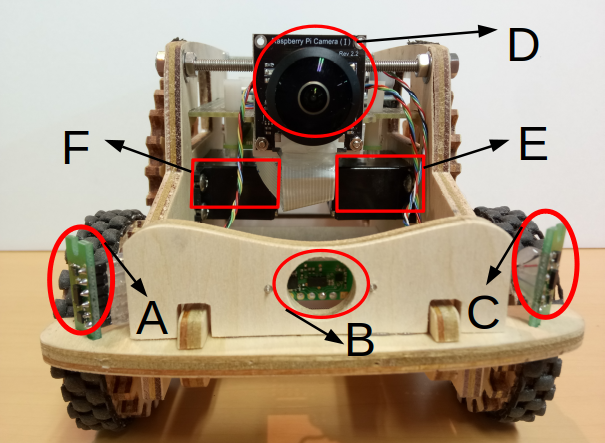
\includegraphics[width=0.9\linewidth]{robot1.jpg}
        \caption{正面図, A:右の距離センサー;
                 B:中央の距離センサー;
                 C:左の距離センサー;
                 D:カメラ(使っていない);
                 E:右モーター;
                 F:左モーター;
                 左右センサー角度:45\degree;
                 ロボット幅:13.5cm;ロボット長さ:20.2cm;ロボット高さ:12.2cm;
        }
    %\end{minipage}
    %\begin{minipage}{0.48\linewidth}
    %    \centering
    %    \includegraphics[width=0.9\linewidth]{robot2.jpg}
    %    \caption{俯瞰図}
    %\end{minipage}
\end{figure}
%\vspace{-6mm}
%\begin{figure}[h]
%        \centering
%        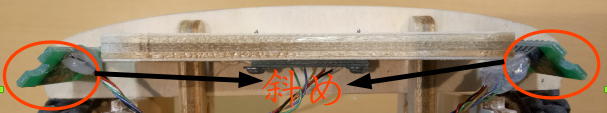
\includegraphics[width=1.0\linewidth]{robot4.jpg}
%        \caption{左右のセンサー角度表示}
%\end{figure}




\section{ニューラルネットワーク}
\subsection{教師データの収集}

一次元画像データとは,二次元(Red,Green,Blue)の画像データの列をそれぞれ足し算して,
得た3つのベクトルをくっつけることである(\ref{eq:onedimension}式参照).
$\boldsymbol R_{\rm i}$,$\boldsymbol G_{\rm i}$,$\boldsymbol B_{\rm i}$は画像データのRed,Green,Blueそれぞれの約130行目から200行目
,70行の行列,$i$は列の番号,$N$は列の数(本研究は$N$=320),$\vec u$は$1$行$960$列のベクトル.

Fig.\ref{roboteye}はロボットの視点,コース以外とロボット自分を映ってる部分がトリミングする.

\vspace{-2mm}
\begin{eqnarray}
\left\{
\begin{aligned}
\vec u_{\rm r}= \sum_{i=1}^N \boldsymbol R_{\rm i}\\
\vec u_{\rm g}= \sum_{i=1}^N \boldsymbol G_{\rm i}\\
\vec u_{\rm b}= \sum_{i=1}^N \boldsymbol B_{\rm i}\\
%begin{array}
%\vec u = \vec u_{\rm r} & \vec u_{\rm g} & \vec u_{\rm b} \\
%end{array}
\vec u = (\vec u_{\rm r},\vec u_{\rm g},\vec u_{\rm b}) \\
\end{aligned}
\right.
\label{eq:onedimension}
\end{eqnarray}


\subsubsection{大きいハンドルで教師データ収集}
教師データは,コースに障害物(他のロボット,Fig.\ref{data_colle}の黒い円囲まれてないロボット)をコースの中にランダムに置いて,
データ収集ロボットをラジコンして,障害物と壁を避けながら時計回りと反時計回り両方走行して,教師データ収集する.
障害物の位置もランダムに変更して,合計3000個教師データ収集した.

ラジコンの方法はtable\ref{radio_rule}の大きいハンドルの部分を参照して,
"D"以外のボタンを押す瞬間の画像データを一次元画像データに変更して,
ソケット通信で学習用パソコンに送信して,教師データの収集を行う.
大きいハンドルというのは,ボタン"J"と"L"押すと,
モーターの出力が35単位変えるということである.
\subsubsection{小さいハンドルで教師データ収集}
小さいハンドルで教師データ収集は大きいハンドルで教師データ収集と同じコースで収集する
,障害物については,止まってるロボット約6台,感覚運動写像より走行するロボット1台,
別の人がラジコンするロボット2台の環境で,データ収集ロボットをラジコンして,
障害物と壁を避けながら時計回りと反時計回り両方走行して,教師データ収集する.
合計6000個教師データ収集した.

ラジコンの方法はtable\ref{radio_rule}の小さいハンドルの部分を参照して,
ボタンを押す瞬間の画像データを一次元画像データに変更して,
ソケット通信で学習用パソコンに送信して,教師データの収集を行う.
小さいハンドルというのは,ボタン"J"と"L"押すと,モーターの出力が15単位変えるということである.

\begin{table}[!ht]
\setlength\tabcolsep{1pt}
\begin{center}
\begin{tabular}{|c|c|c|c|c|}
\hline
 & \multicolumn{2}{|c|}{小さいハンドル} & \multicolumn{2}{c|}{大きいハンドル}\\
\hline
 & Left motor & Right motor & Left motor & Right motor \\
\hline
W & +20 & +20 & +35 & +35\\
\hline
S & -15 & -15 & -35 & -35\\
\hline
A & * & * & -56 & -56\\
\hline
D & * & * & =0 & =0 \\
\hline
J & -15 & +15 & -0 & +35 \\
\hline
L & +15 & -15 & +35 & -0 \\
\hline
K & \multicolumn{4}{|c|}{操作JとKで変化した出力が0になる} \\
\hline
\end{tabular}
\end{center}
\caption{
大きいハンドルと小さいハンドルの違い
}
\label{radio_rule}
\end{table}



\vspace{-2mm}
\begin{figure}[h]
        \centering
        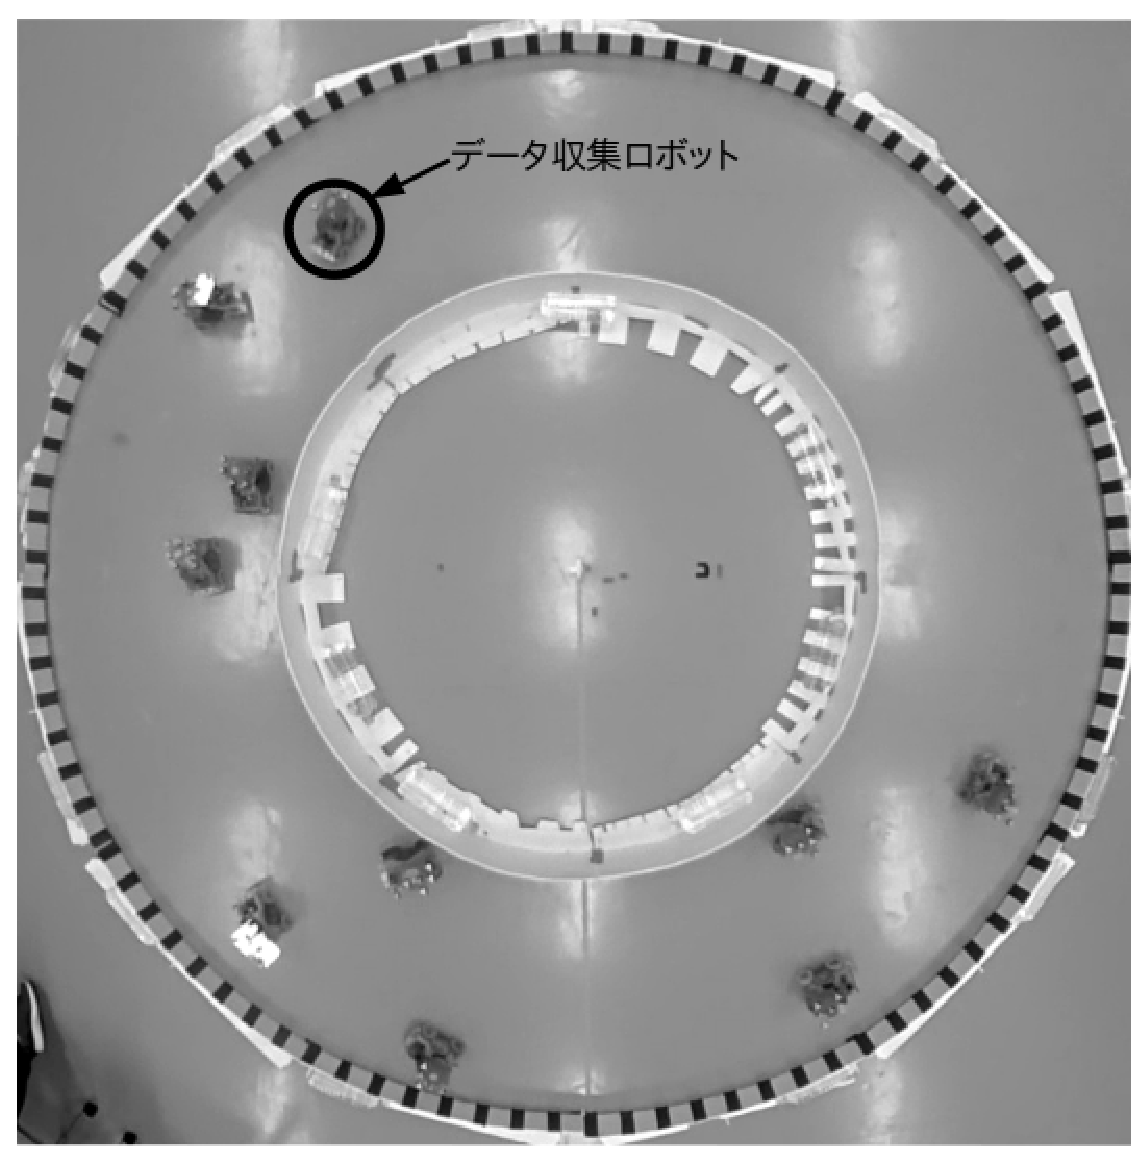
\includegraphics[width=0.8\linewidth]{teacher_collection.eps}
        \caption{データ収集}
        \label{data_colle}
\end{figure}

\vspace{-5mm}
\begin{figure}[h]
\centering
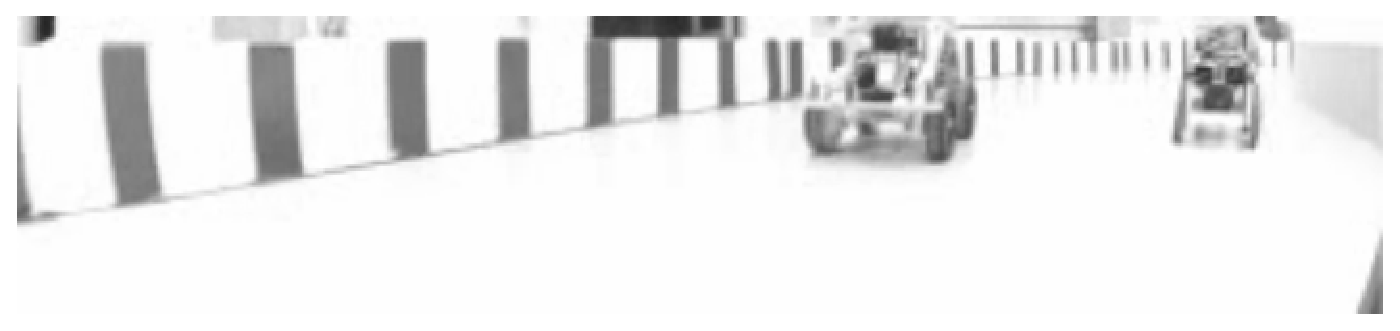
\includegraphics[width=0.7\linewidth]{robot_eye.eps}
\caption{ロボットの視点}
\label{roboteye}
\end{figure}




\subsection{データの学習}
入力層:ニューロン数は960(一次元画像データの値の数).

中間層:ニューロンの数を100から1100まで変更して,シミュレーションした.Fig.\ref{anti_left}の横軸は中間層ニューロンの数,
縦軸は左のモーターの予測出力と教師データ出力の平均二乗誤差.
Fig.\ref{anti_right}の横軸は中間層ニューロンの数,縦軸は右のモーターの予測出力と教師データ出力の平均二乗誤差.
中間層のニューロンの数の増加に従って,回帰誤差の増減に規則性はみられない.
経験によって,中間層のニューロンの数を1000にした.

出力層:左右のモーターの制御パワーを計算するので,出力層ニューロンの数が2にする.

活性化関数:relu関数.

最適化アルゴリズム:Adamでバッチ学習である.

Adamのパラメーター: $\alpha$=0.01,$\eta$=0.3,$\beta$1=0.9,$\beta$2=0.9,$\epsilon$=$1\times e^{-8}$.$w$=0.

Fig.\ref{LeftOutput}とFig.\ref{rightOutput}は学習終わったニューラルネットワークの回帰結果部分的グラフです.
横軸はデータの番号(1番目から600番目の教師データをグラフした),
縦軸は左のモーターの出力(Fig.\ref{LeftOutput})と右のモーターの出力(Fig.\ref{rightOutput})です.
%オレンジ色の線が教師データの出力で,青色線が教師データと同じの入力(1次元画像データ)でニューラルネットワークの予測出力です.
ニューラルネットワークの予測出力が教師データの出力に完璧に回帰していないと見られるけど,
人間のラジコンで収集した教師データも完璧ではないと考えて,ある程度回帰できれば,実際の走行実験の振舞いで評価するにした.

\vspace{-2mm}
\begin{figure}[h]
        \centering
        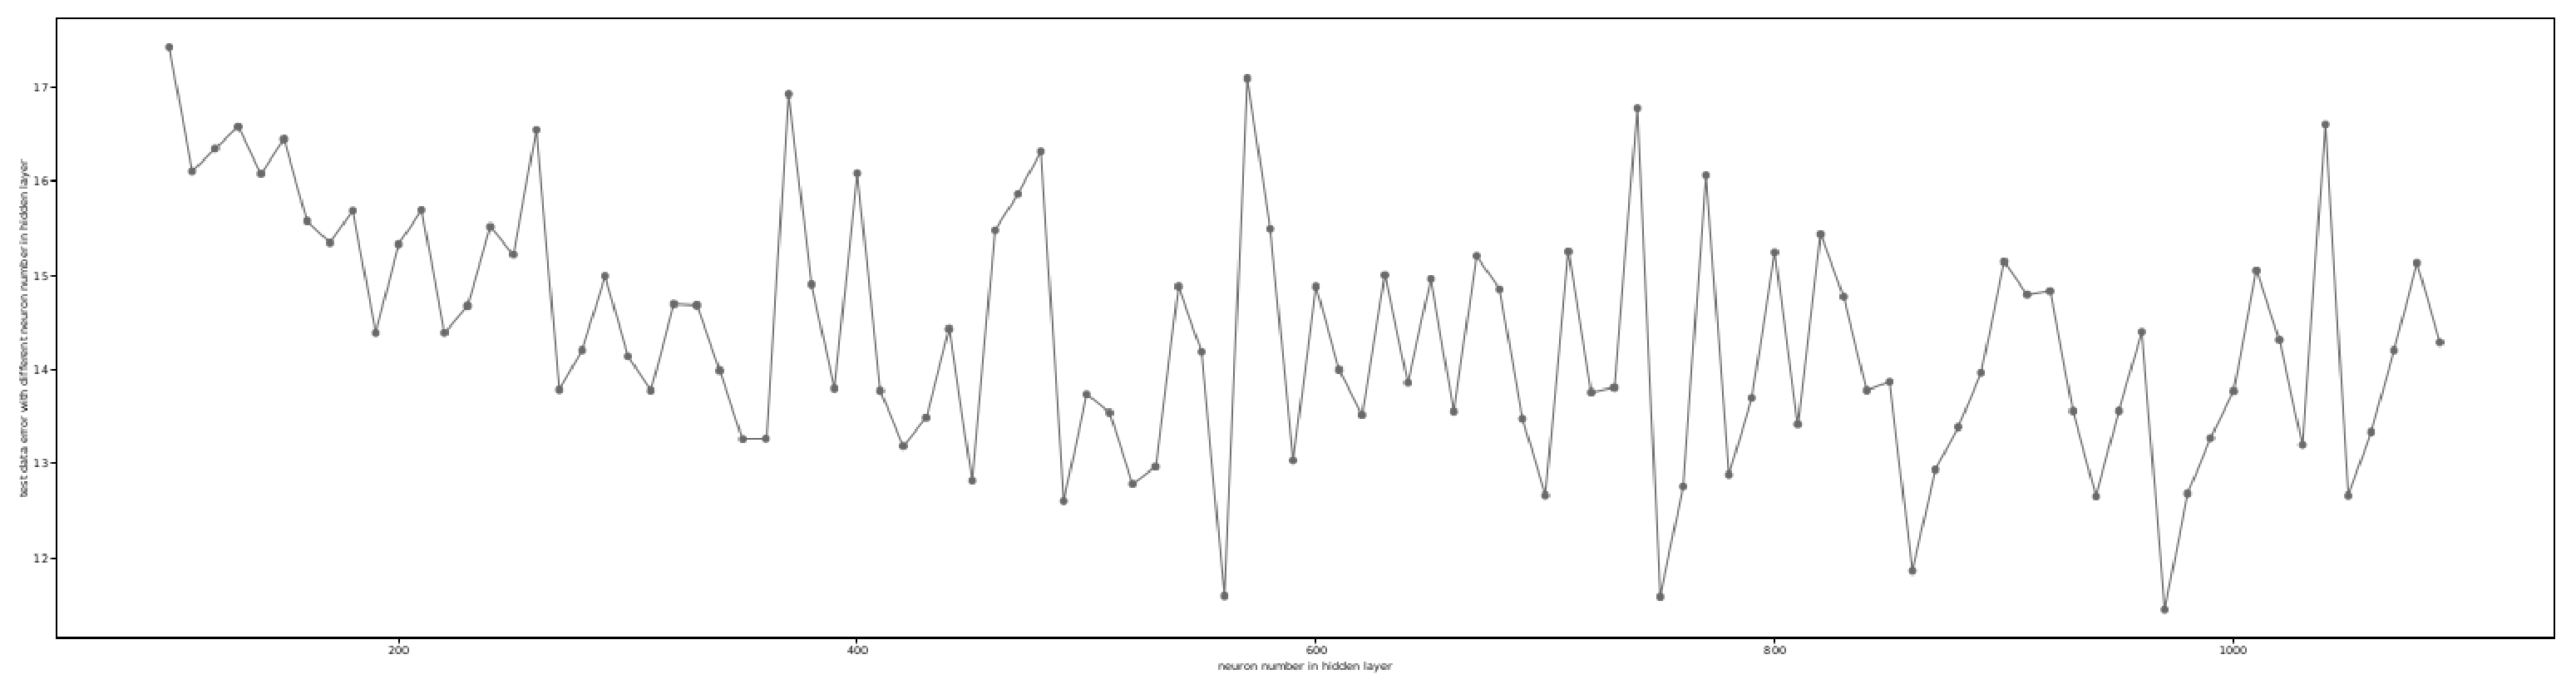
\includegraphics[width=1.0\linewidth]{anti_left.eps}
        \caption{中間層ニューロンの数と左のモーターの出力誤差}
        \label{anti_left}
\end{figure}
\vspace{-5mm}
\begin{figure}[h]
        \centering
        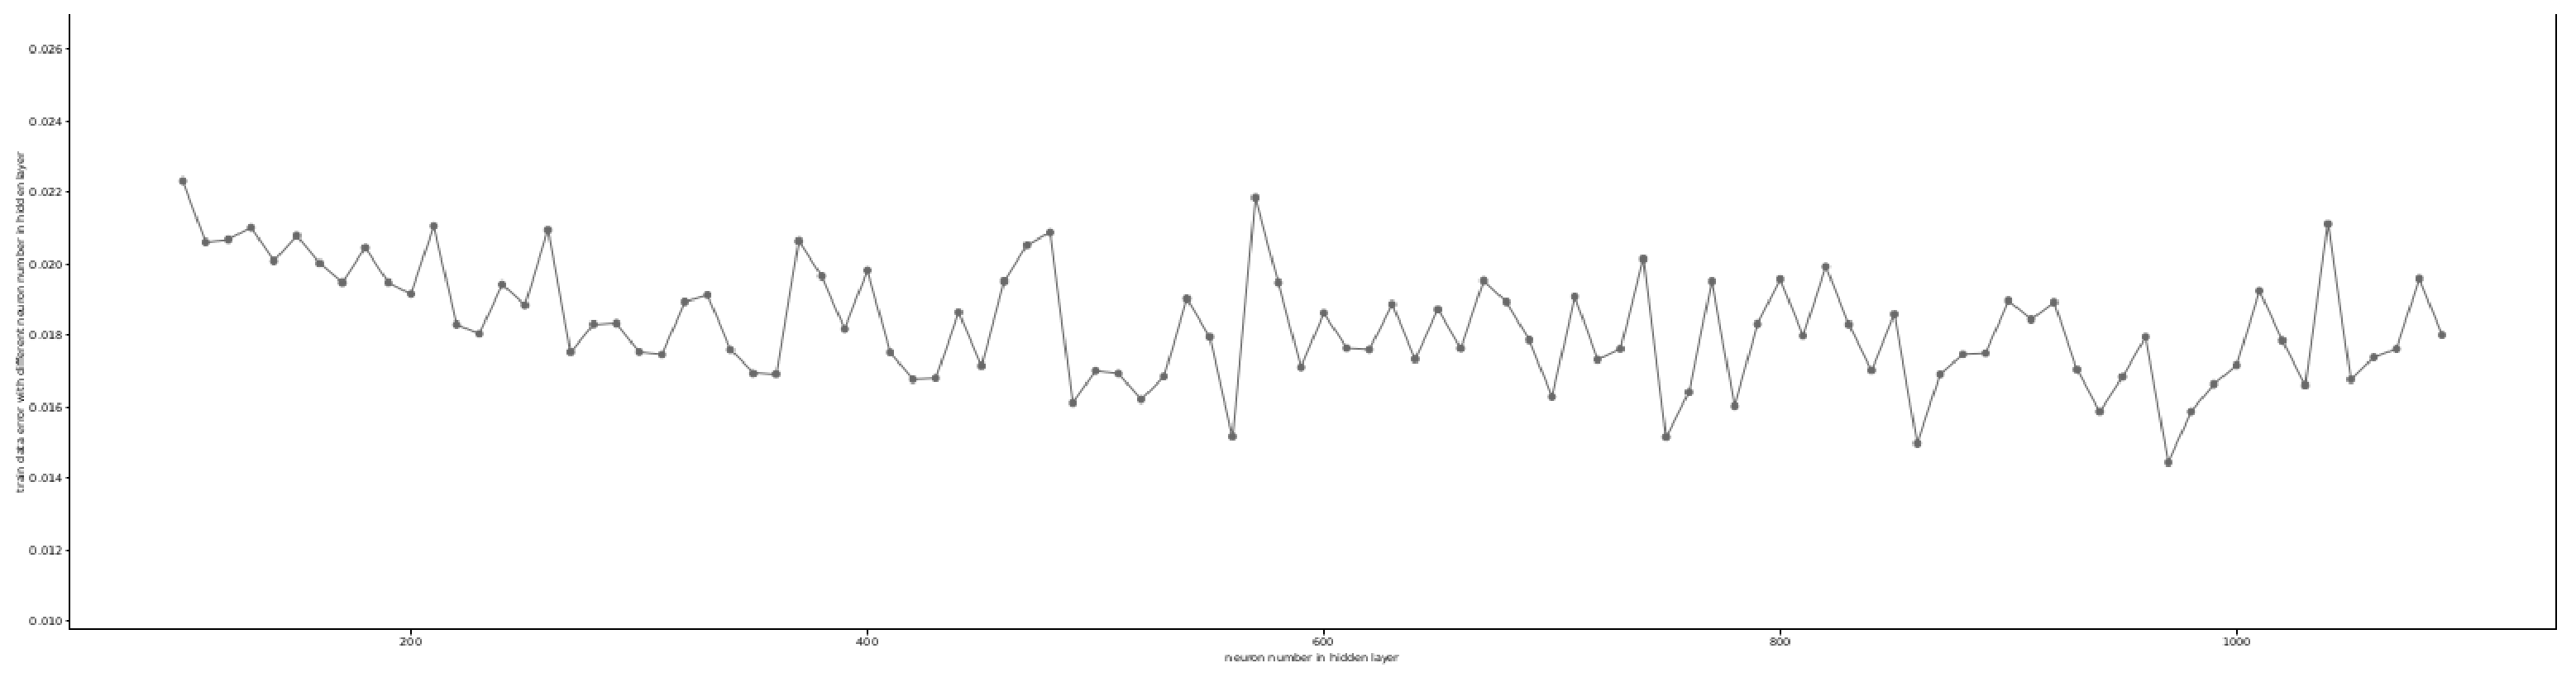
\includegraphics[width=1.0\linewidth]{anti_right.eps}
        \caption{中間層ニューロンの数と右のモーターの出力誤差}
        \label{anti_right}
\end{figure}

\vspace{-7mm}
\begin{figure}[!ht]
    \centering
    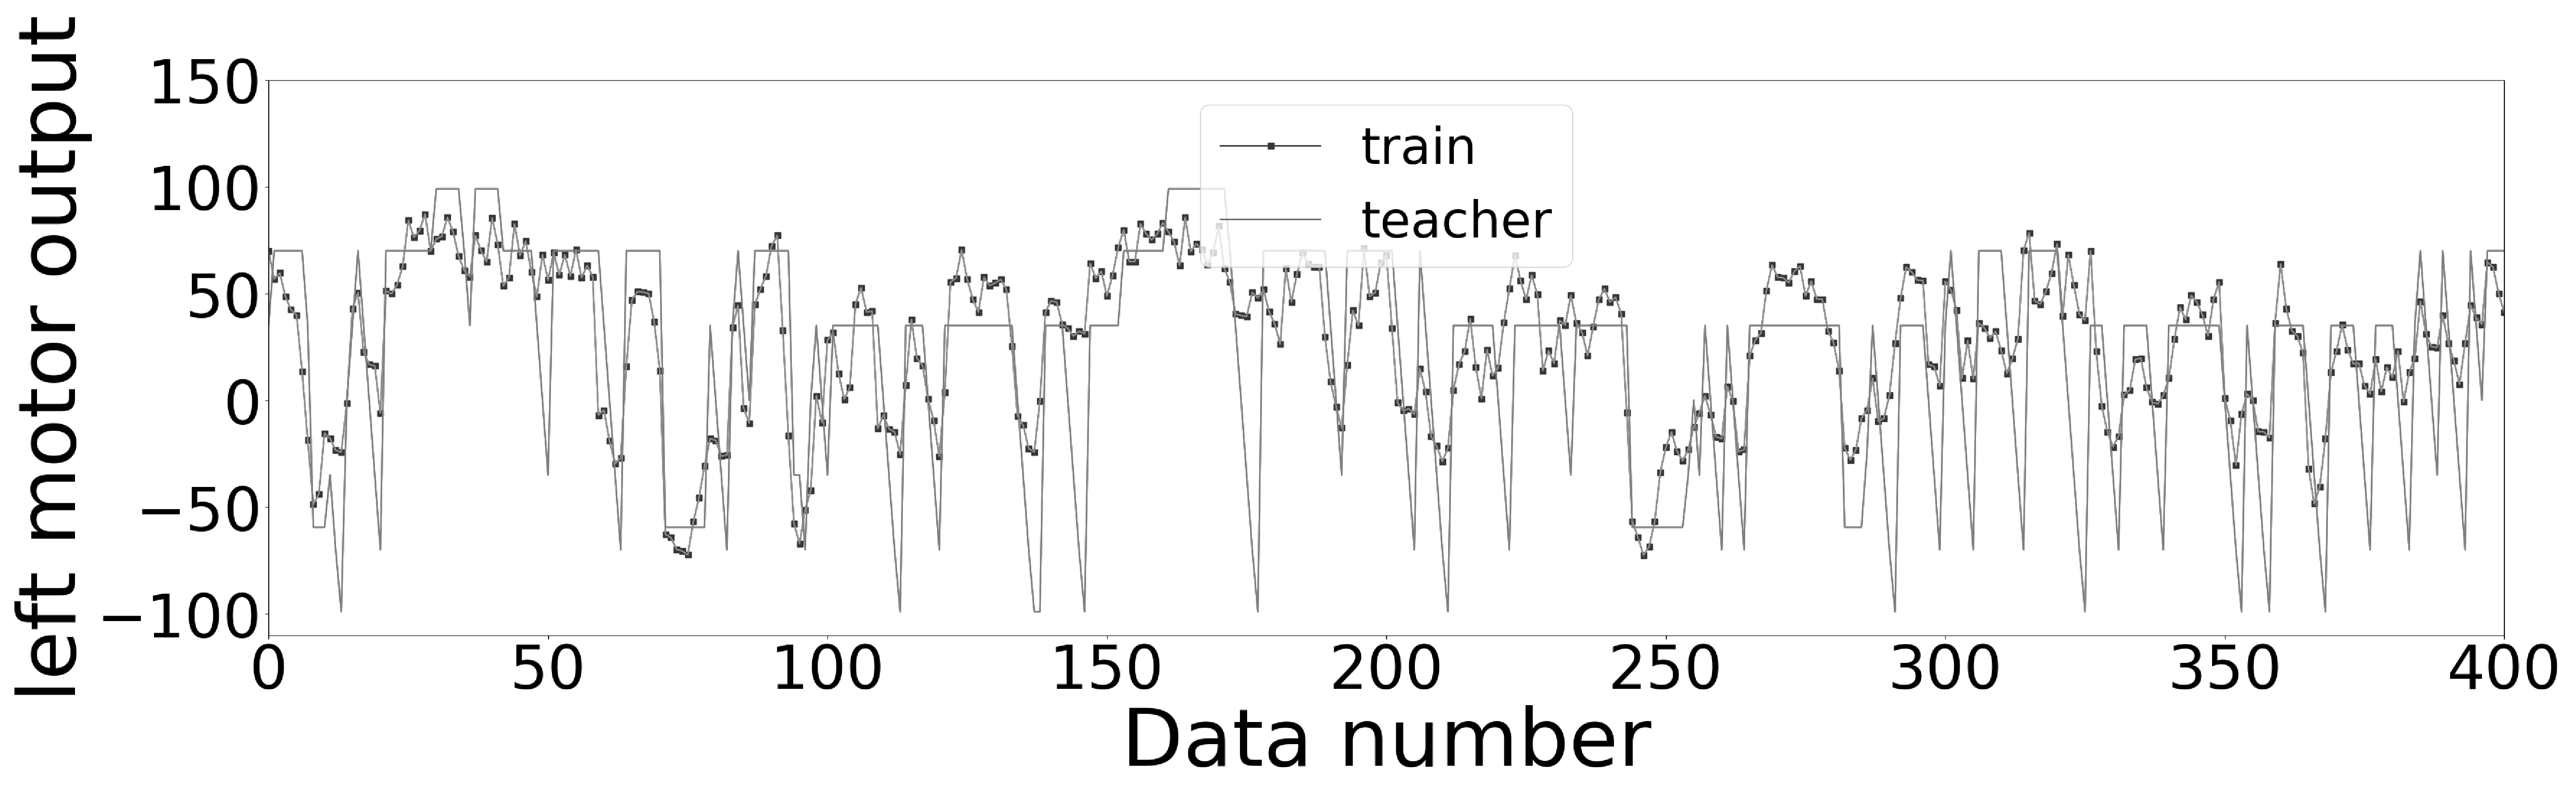
\includegraphics[width=1.0\linewidth]{LeftOutput.eps}
    \caption{NNで左のモーターの出力の回帰結果(局部)}
    \label{LeftOutput}
\end{figure}

\vspace{-7mm}
\begin{figure}[!ht]
    \centering
    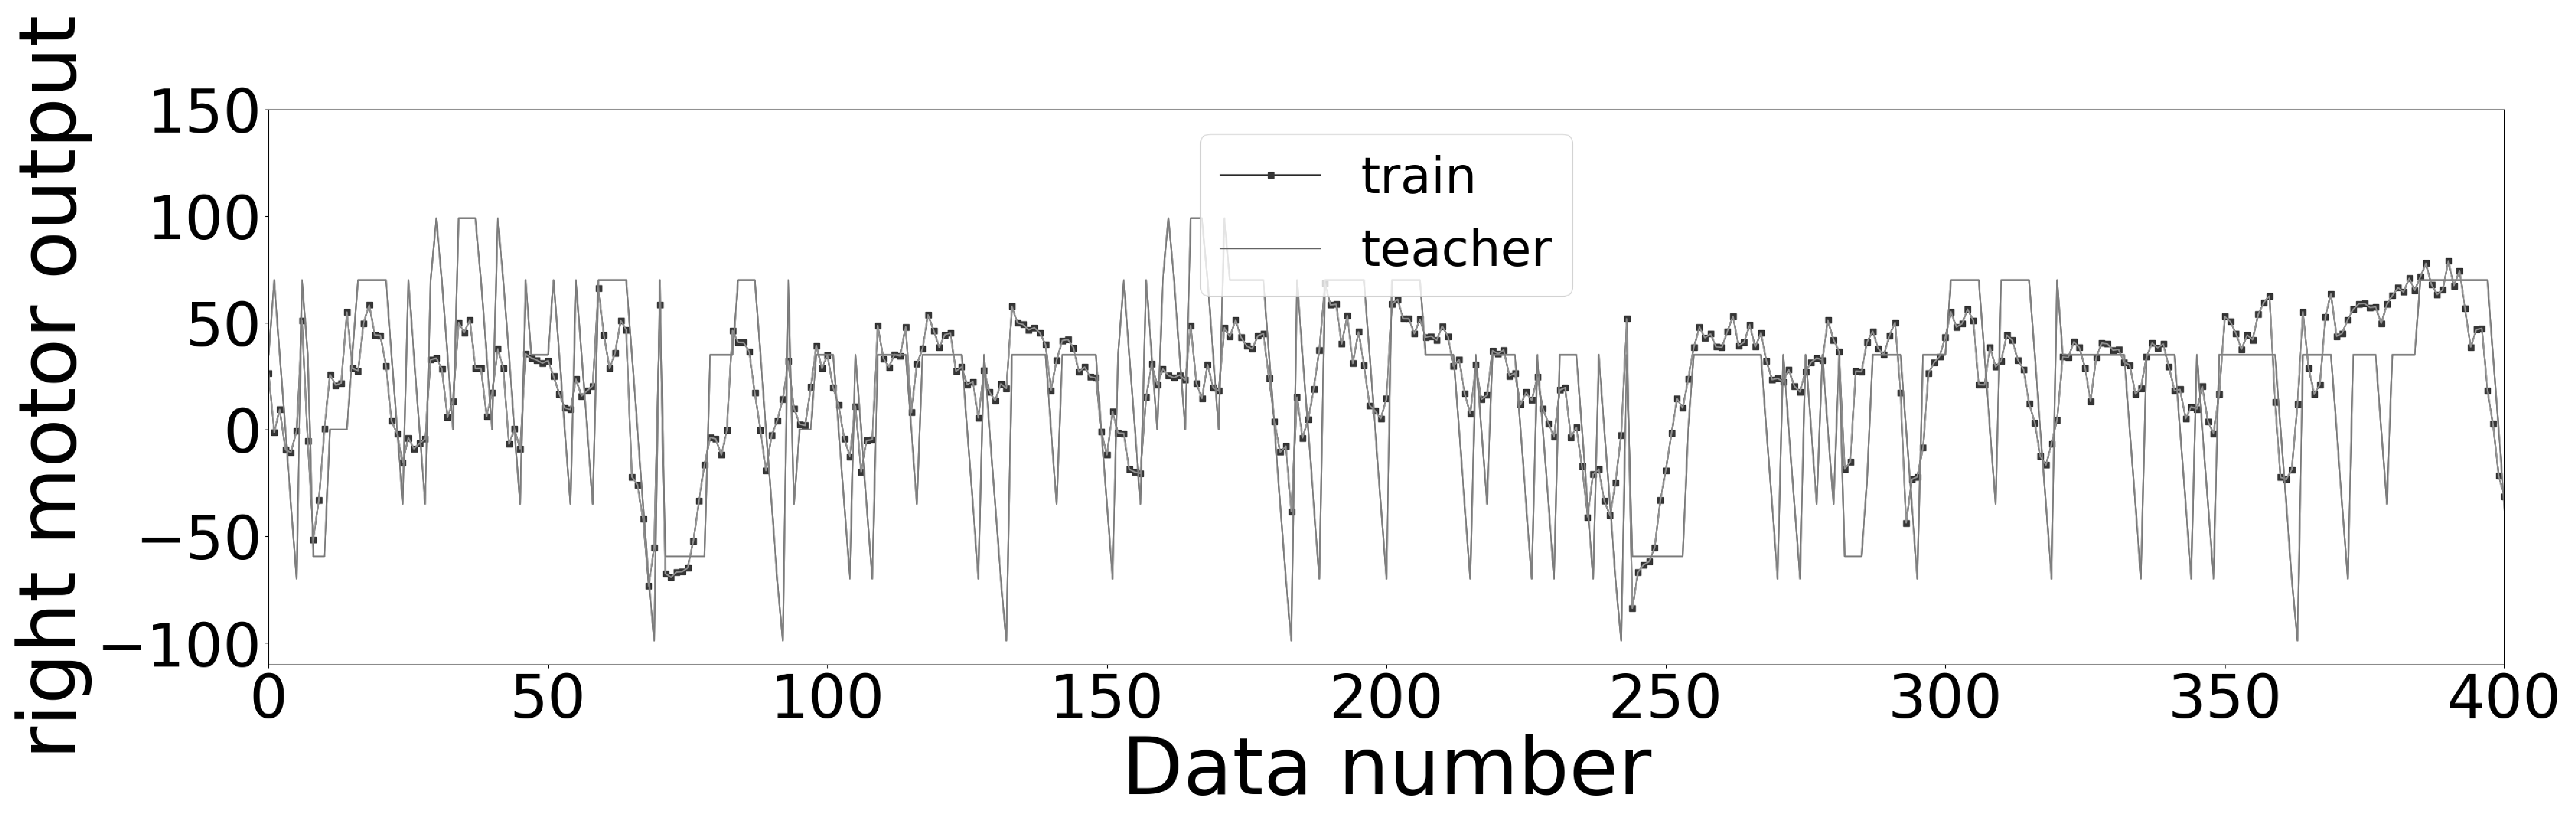
\includegraphics[width=1.0\linewidth]{rightOutput.eps}
    \caption{NNで右のモーターの出力の回帰結果(局部)}
    \label{rightOutput}
\end{figure}

\section{感覚運動写像}
感覚運動写像とは,センサー値を変数とする関数によってモーターの出力を決定することであり,
その瞬間のセンサー値だけを使う,最も単純な反応行動のための知能の一つである\cite{asada}.
本研究では,非線形感覚運動写像モデル(式(\ref{eq:mR})と式(\ref{eq:mL}))が使われている.

3つの距離データを相乗平均する得られた$x_{\rm L}$と$x_{\rm R}$を式(\ref{eq:mR})と
式(\ref{eq:mL})に代入して,ロボットの右モーターの出力($m_{\rm R}$)と左モーターの
出力($m_{\rm L}$)を計算する.
$b$は$\tanh$曲線の変曲点であり,実験ではロボット曲がるの反応距離或いは障害物をぶつからない安全距離である.
今回の実験のパラメーターは
$\alpha=35\%$とする.
すなわちロボットは最高速度の70\%の速度で走行する.ニューラルネットワーク教師データ収集ラジコンする時の最高速度と同じです.
$\beta_1=0.004$,
$\beta_2=10$,
$c=0$とする.
詳しい内容は参考文献\cite{li}を参考してください.

\begin{eqnarray}
\begin{aligned}
  m_{\rm R} = &\alpha \tanh(\beta_1(x_{\rm L} - b_{\rm L})) + \\
        &\alpha \tanh(\beta_2(x_{\rm L} - b_{\rm L})) + c
 \label{eq:mR}
\end{aligned}
\end{eqnarray}

\begin{eqnarray}
\begin{aligned}
  m_{\rm L} = &\alpha \tanh(\beta_1(x_{\rm R} - b_{\rm R})) + \\
        &\alpha \tanh(\beta_2(x_{\rm R} - b_{\rm R})) + c
 \label{eq:mL}
\end{aligned}
\end{eqnarray}

\section{走行実験}
本文は円形コースで実験する.
時計回りロボット4台と反時計回りロボット4台を2つずつセットにしてコースの中にランダムに置いて,
約8分間実験した.ロボットが自分の向きを判断できるため,
内側のコース壁を青色に塗って,
外側のコース壁を青色の縞模様としている.

ロボットが破線1から反時計回りで破線2まで移動して,$\theta$が0から$\pi$に変わる.
破線1から時計回りで破線2まで移動して,$\theta$が0から$-\pi$に変わる.
$R$はロボットからコース中心までの距離である(図\ref{courseshitar}).
それに,ロボットが反時計回りで破線1を通過したら,通過回数$n_{ij}$が+1,
ロボットが時計回りで破線1を通過したら,通過回数$n_{ij}$が-1になる.
次,ロボット一台ずつ,各自の$n_{ij}$を計測して,
各ロボットの通過回数の絶対値を足し算して,1回の実験の通過回数になる.
(\ref{eq:flow})式で$i$番目の実験の流量$Q_i$を求めて,
(\ref{eq:flow_ave})式で流量の平均値を求める.
$j$はロボットの番号で,
$k$はロボットの台数です(今回の実験で1から8まで合計8台ロボットを使ったので,$k=8$.
$T_i$は$i$番目の実験の1方向走行流になる時間です(先行研究\cite{li}の$T_{\rm 1d}$と同じ,単位:min)
$w$がコースの幅(単位:m),
$N_{\rm exp}$は全実験回数を表す.

ロボットが渋滞状態を解消する能力も比較するため,2つロボットをペアとして,
ランダムの初期配置(図\ref{randstart})と渋滞の初期配置(図\ref{crowdstart})の実験を行った

\vspace{-1mm}
\begin{figure}[h]
        \centering
        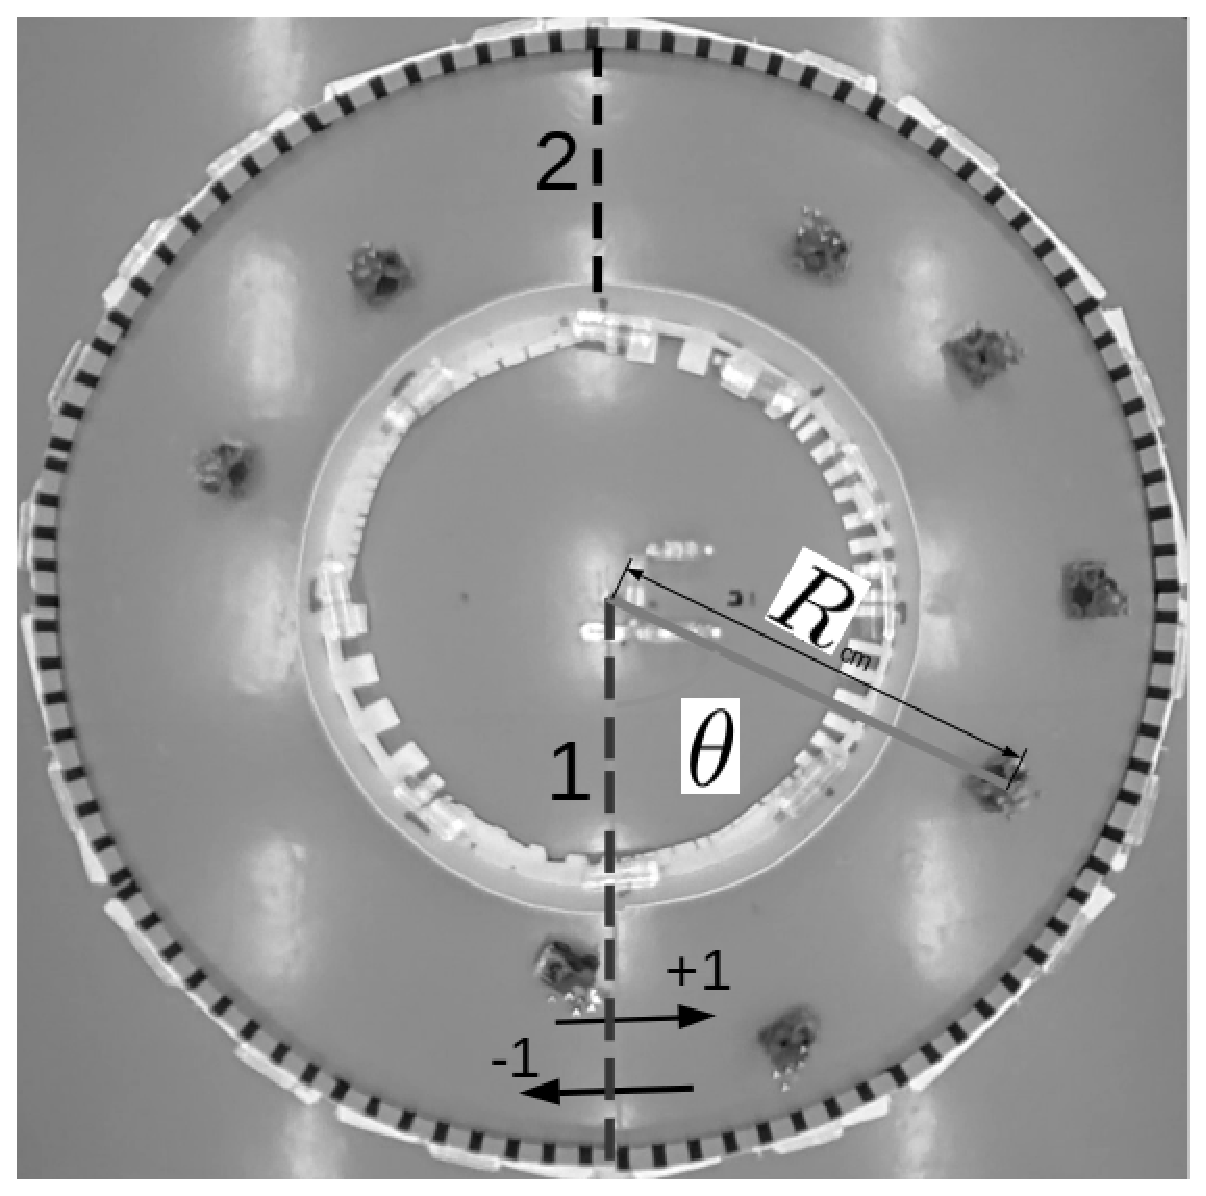
\includegraphics[width=0.6\linewidth]{shitaR.eps}
        \caption{実験の様子(俯瞰図)と$\theta$の説明}
        \label{courseshitar}
\end{figure}

\vspace{-6mm}
\begin{eqnarray}
Q_i &=& \frac{\sum_{j=1}^{k} |n_{ij}|}{wT_i}
\label{eq:flow} \\
\bar{Q} &=& \frac{1}{N_{\rm exp}}\sum_{i=1}^{N_{\rm exp}} Q_i
\label{eq:flow_ave} 
\end{eqnarray}

\vspace{-3mm}
\begin{figure}[h]
    \begin{minipage}{0.49\linewidth}
        \centering
        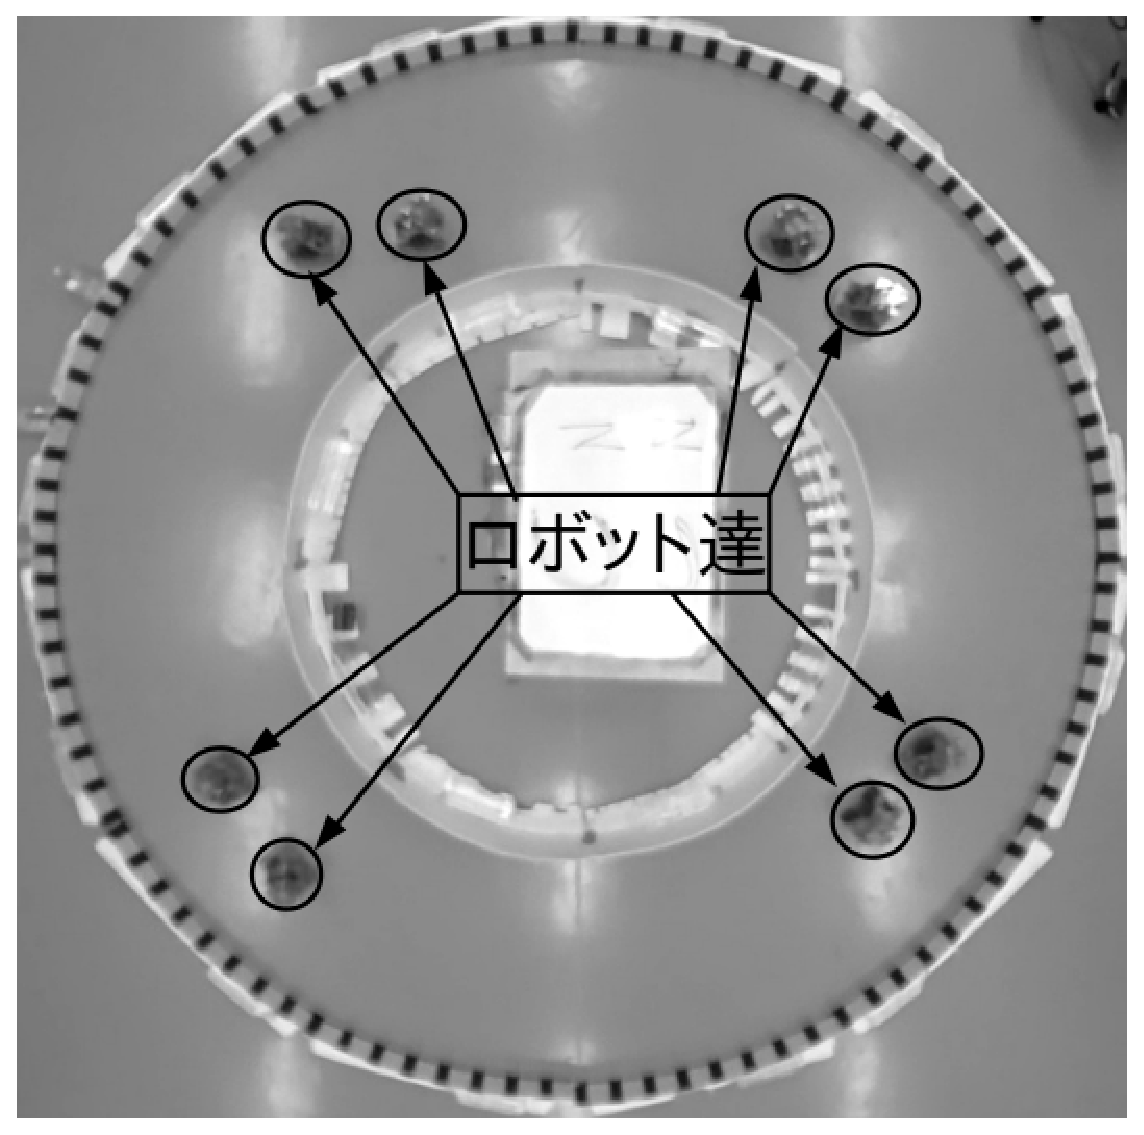
\includegraphics[width=1.0\linewidth]{startrand.eps}
        \caption{ランダムの初期配置}
        \label{randstart}
    \end{minipage}
    \begin{minipage}{0.49\linewidth}
        \centering
        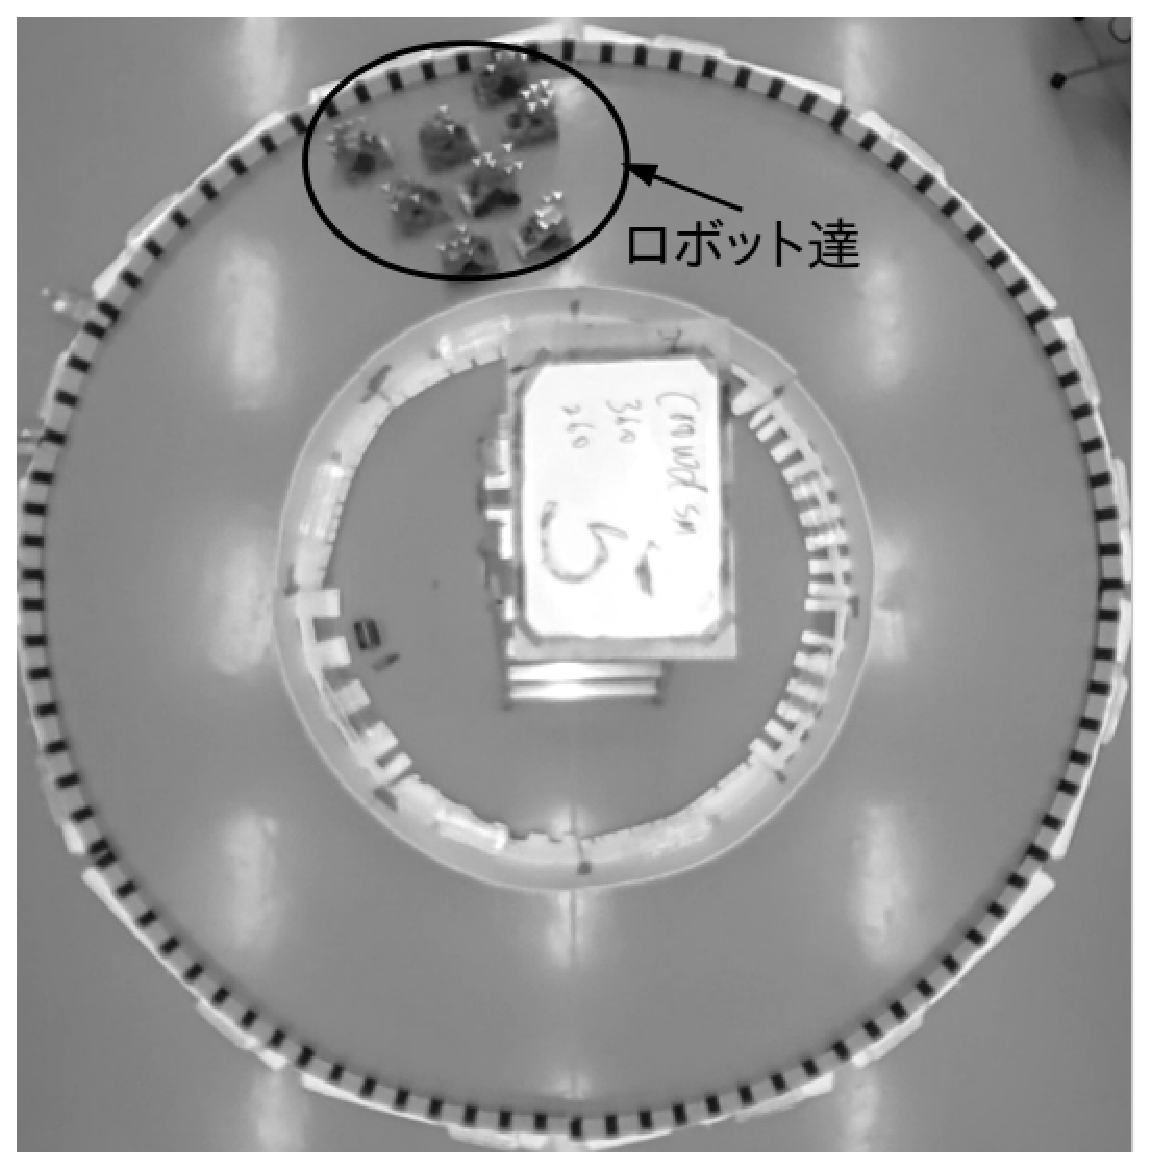
\includegraphics[width=1.0\linewidth]{start_crowd.eps}
        \caption{渋滞の初期配置}
        \label{crowdstart}
    \end{minipage}
\end{figure}

\section{実験結果}
\subsection{小さいハンドル教師データでの走行}
我々はまず小さいハンドル教師データを学習した結果で,
ランダムの初期配置によって8台ロボット対面走行を実験した.
Fig.\ref{handle15_dia}は時間($s$横軸)と$\theta$(縦軸上),$R$(縦軸下)の関係図です.
この実験から,一部のロボット達が短時間の対面走行できると確認したけど,
ロボット同士がぶつかる,壁にぶつかる,引っかかって解消不能,方向転換なども観察された.

例として,左の上から3番目,右の上から2番目と3番目のグラフで,$\theta$の変動が止まって,水平になった,
Fig.\ref{handle15_img}は約400秒$\theta$が水平になる部分に対する実験風景です,
実験からロボットが壁にぶつかって,後退しなくて,止まっちゃう,
2つロボットが引っかかって解消不能になって,止まっちゃうことが観察された.
原因として,曲がりと後退のパワーが弱いと考えて,大きいハンドルのラジコンで教師データを収集して実験した,
実験結果は次に説明する.

\vspace{-1mm}
\begin{figure}[!ht]
    \centering
    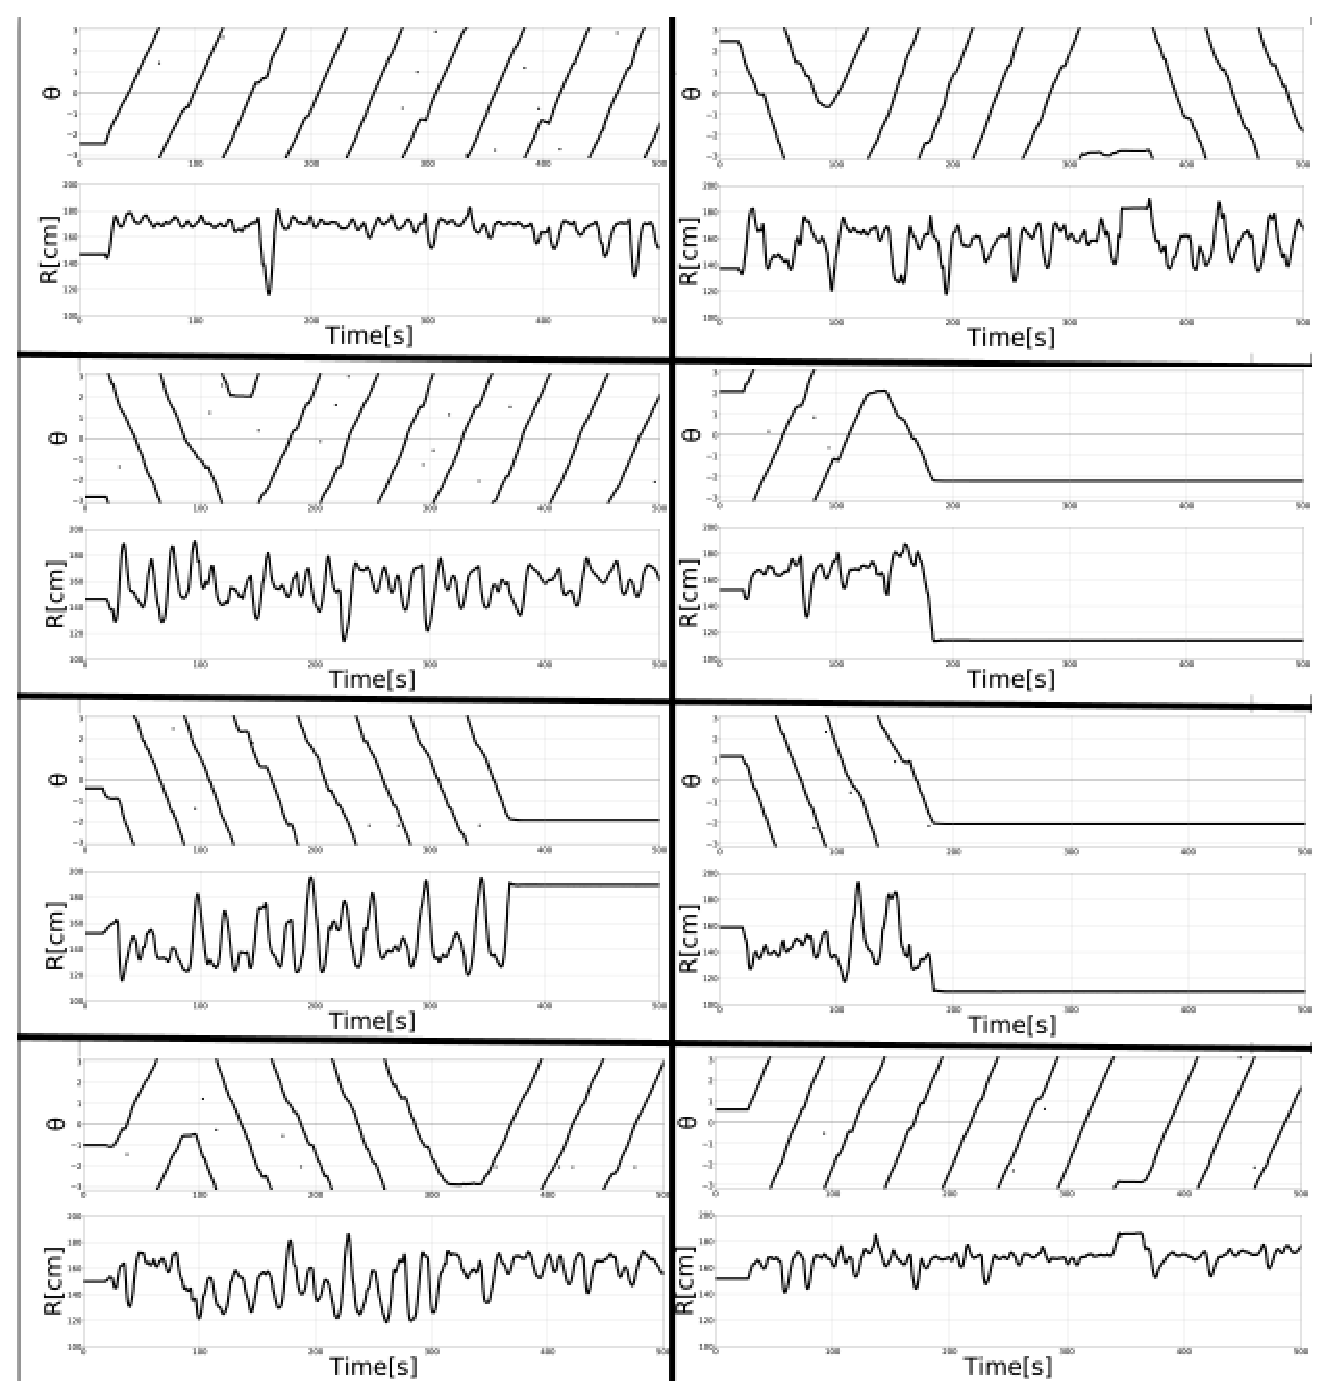
\includegraphics[width=1.0\linewidth]{NN_handle15.eps}
    \caption{小さいハンドルNN,8台ロボットの走行結果}
    \label{handle15_dia}
\end{figure}

\vspace{-5mm}
\begin{figure}[!ht]
    \centering
    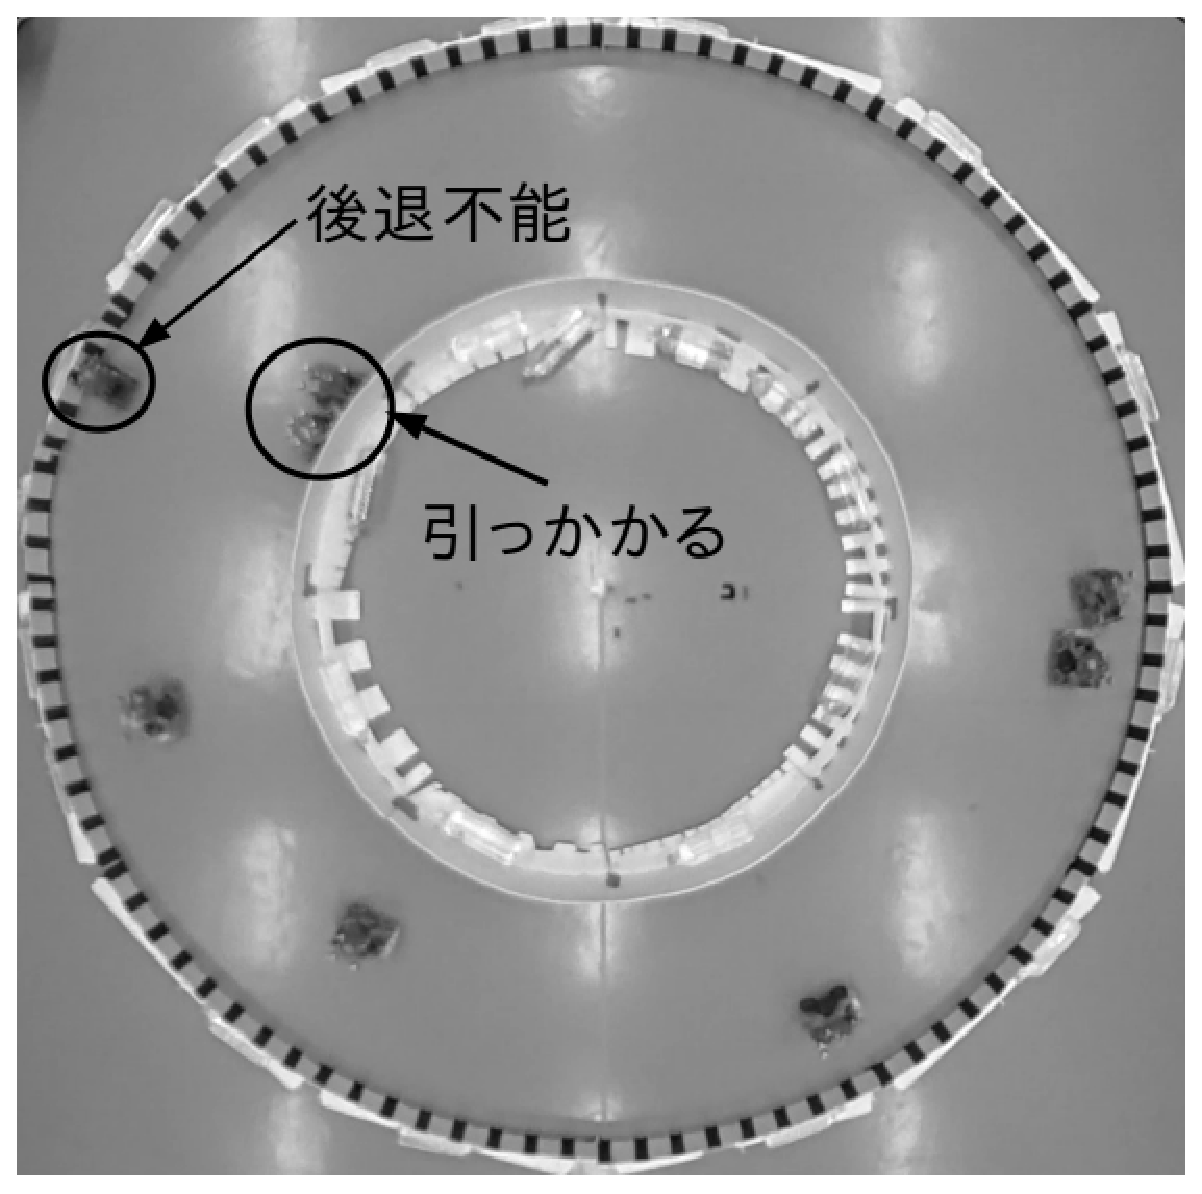
\includegraphics[width=0.6\linewidth]{nnhandle15.eps}
    \caption{小さいハンドルNN走行実験400秒の様子}
    \label{handle15_img}
\end{figure}

\subsection{感覚運動写像と走行の比較}

ラジコンの曲がる値が拡大して(大きいハンドル)収集した教師データの学習結果での自律走行実験も約6回行った.
図\ref{diaRshita}と図\ref{diaRshita_270}はニューラルネットワークにより走行と$b=270,270$の感覚運動写像により
走行の1回の走行実験の時間変化におけるロボット位置の角度($\theta$)と半径($R$)のまとめ図である.
横軸は時間(s),縦軸上のほうが$\theta$,下のほうが$R$である.

この2つグラフから,大きいハンドルでのニューラルネットワークよりの走行のほうが対面走行を最後まで維持でき,
スムーズに走れると観察された(図\ref{NN300},時計回りのロボット達が内側の壁に沿う,反時計回りのロボット達が外側の壁に沿う).

$b=270,270$の感覚運動写像によりの走行のほうが途中に1方交流になった(図\ref{diaRshita_270},
約250秒からすべての$theta$の曲線が右に傾斜する),
$R$の変動範囲が大きい(衝突が多い),1方向走行流になったら,$R$の変動も安定になって,
外側の壁に沿って反時計回り走ると観察された(図\ref{SMM300}).


\vspace{-1mm}
\begin{figure}[!ht]
    \centering
    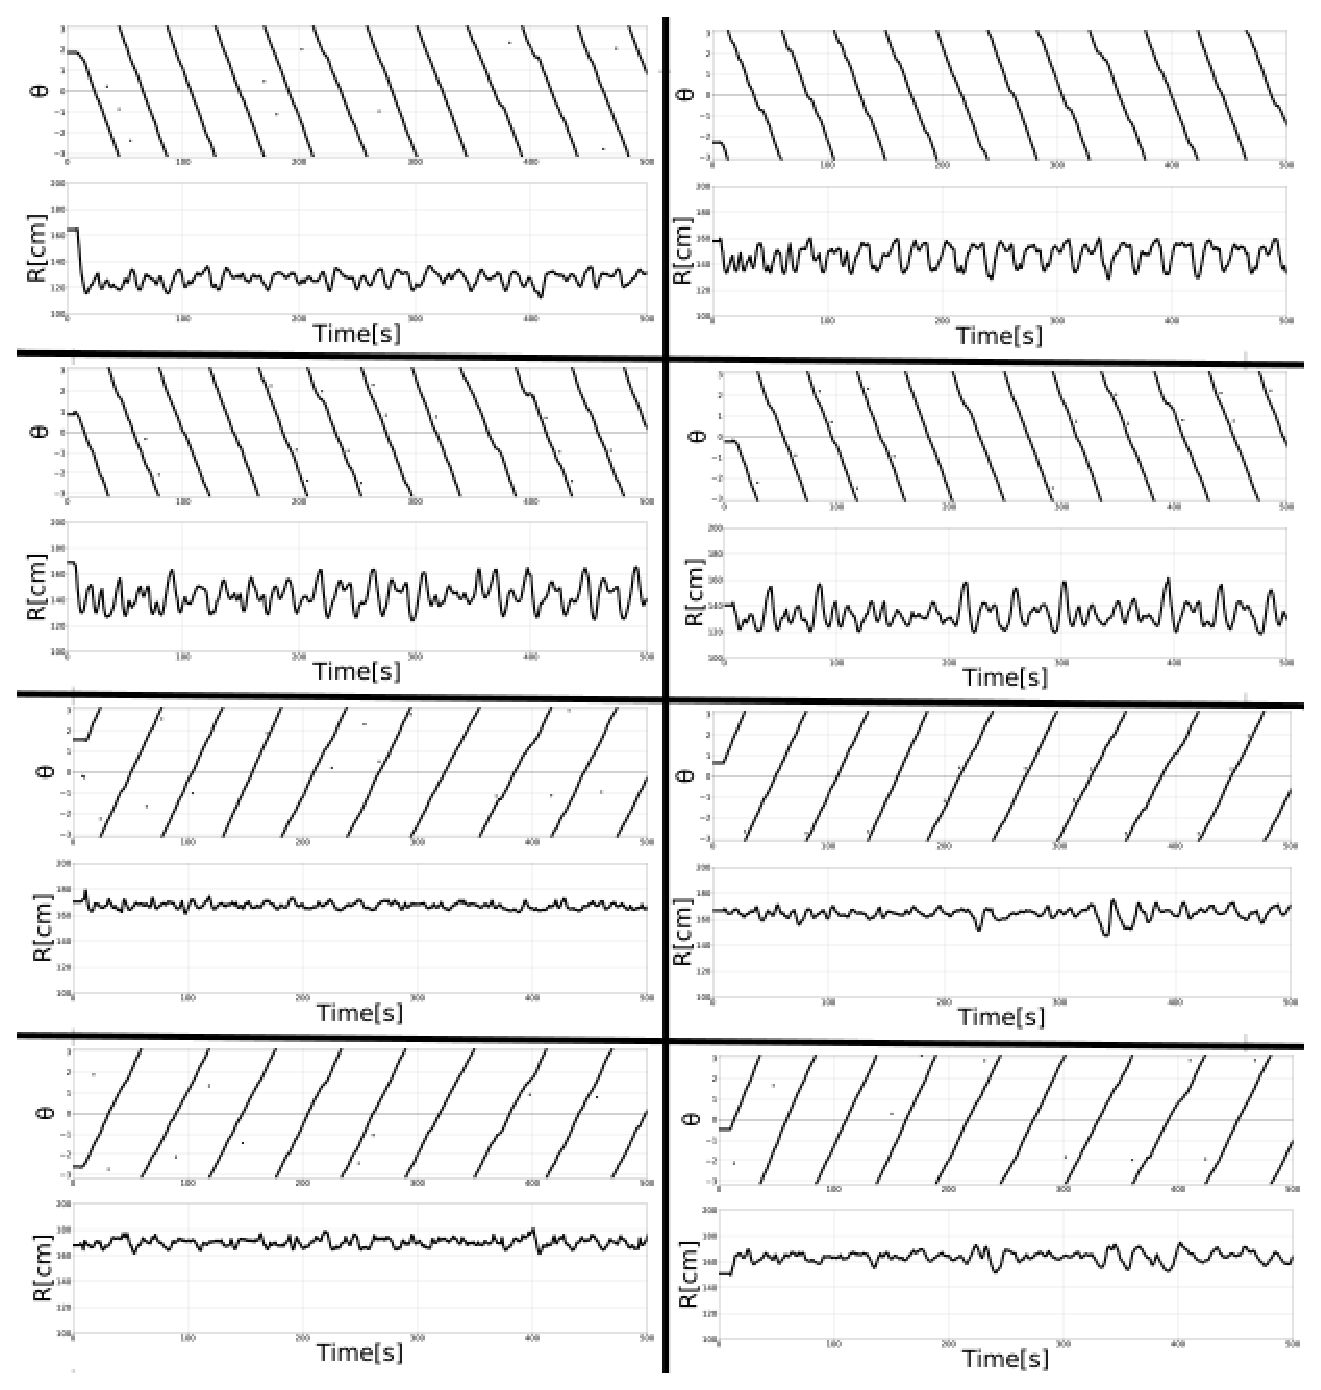
\includegraphics[width=1.0\linewidth]{nn_shita_R_rand.eps}
    \caption{ランダムの初期配置でNNにより走行の$\theta$,$R$と時間の関係図}
    \label{diaRshita}
\end{figure}

\vspace{-4mm}
\begin{figure}[!ht]
    \centering
    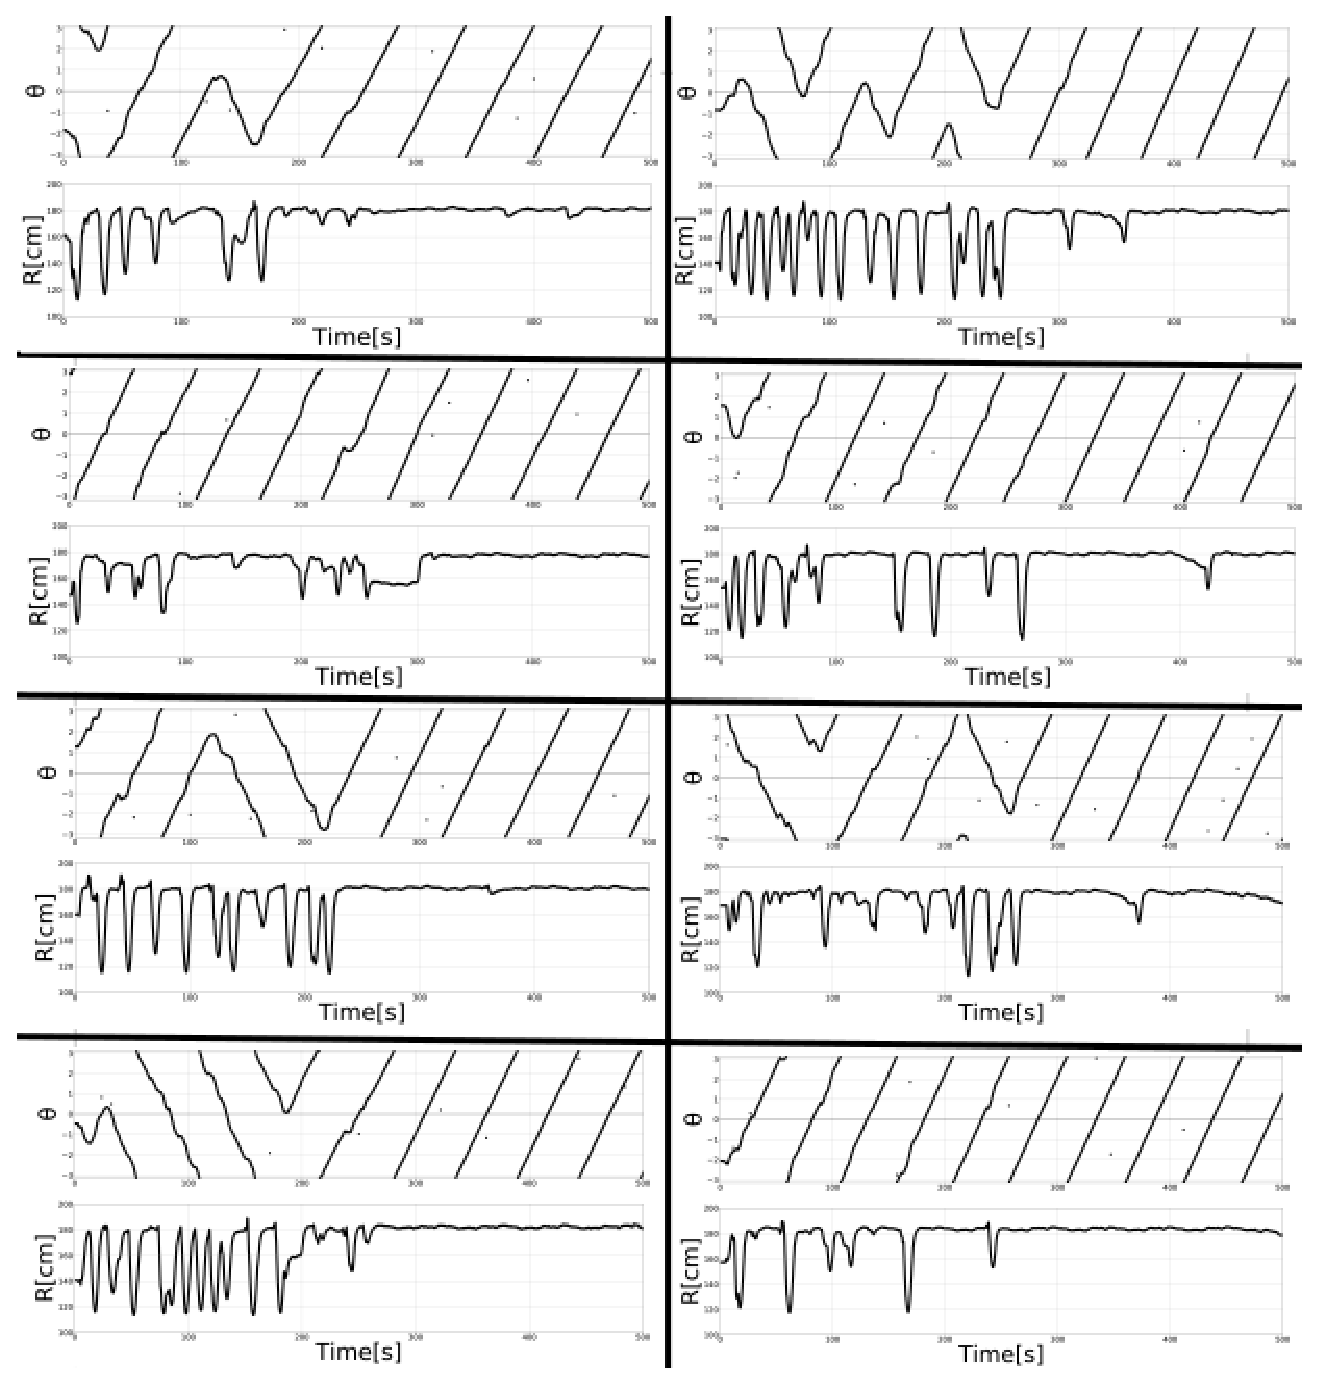
\includegraphics[width=1.0\linewidth]{smm_shita_R_rand270.eps}
    \caption{ランダムの初期配置でSMMにより走行の$\theta$,$R$と時間の関係図}
    \label{diaRshita_270}
\end{figure}

\begin{figure}[h]
    \begin{minipage}{0.48\linewidth}
        \centering
        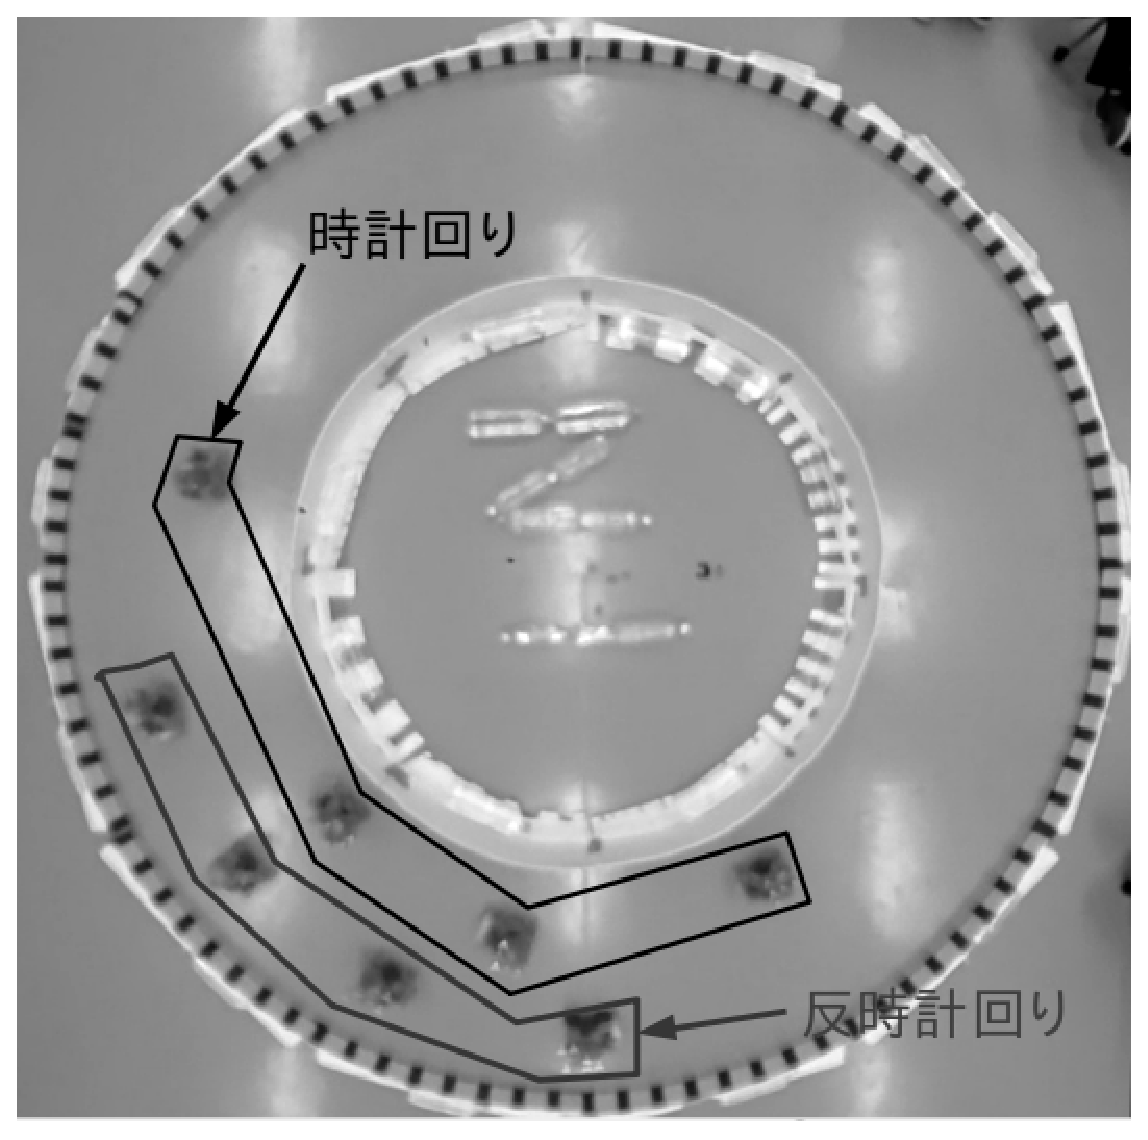
\includegraphics[width=1.0\linewidth]{NN_exp.eps}
        \caption{300秒neural network走行風景}
        \label{NN300}
    \end{minipage}
    \begin{minipage}{0.48\linewidth}
        \centering
        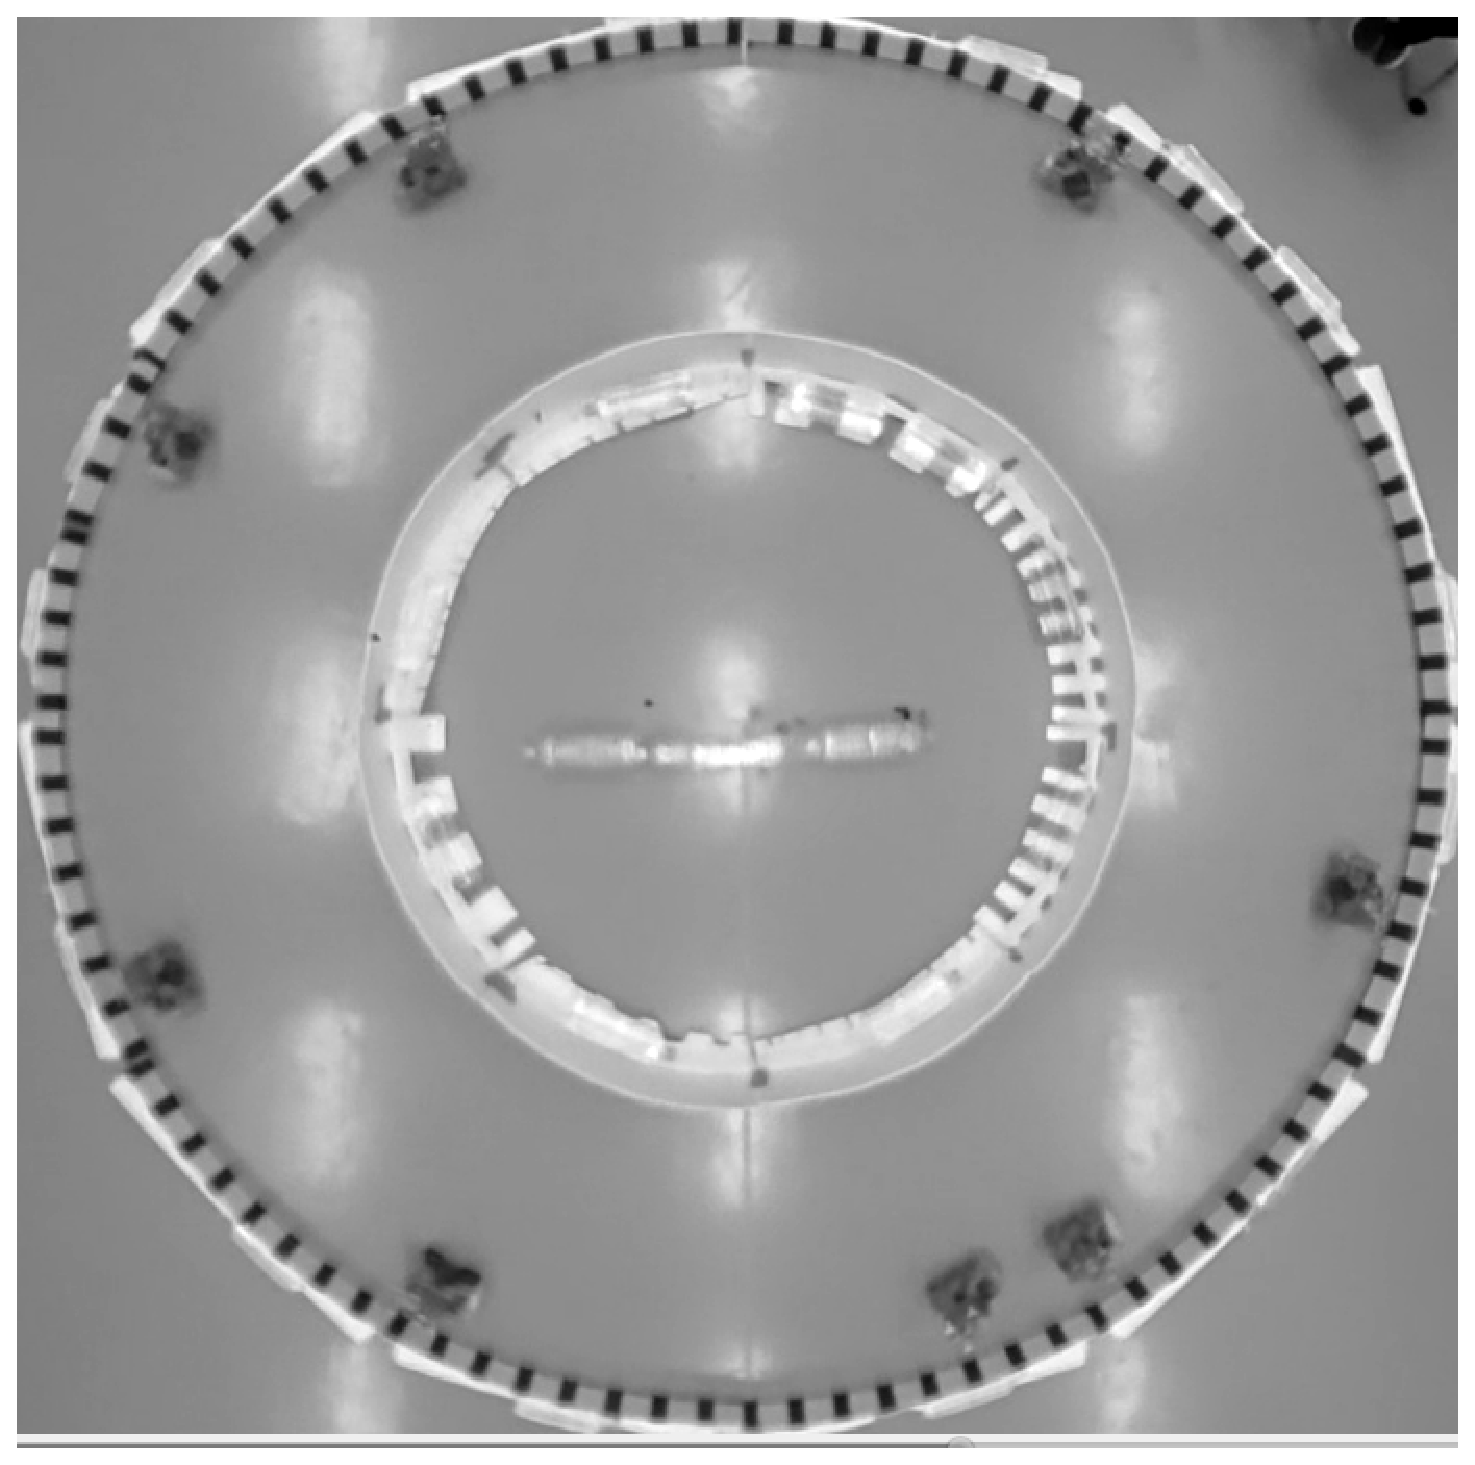
\includegraphics[width=1.0\linewidth]{SMM270_exp.eps}
        \caption{300秒感覚運動写像走行風景}
        \label{SMM300}
    \end{minipage}
\end{figure}

\subsection{感覚運動写像と流量の比較}
流量を比較するため,ランダムと渋滞,2種類の初期配置でニューラルネットワークより,感覚運動写像より約5回実験した.
Fig.\ref{random_result}とFig.\ref{crowd_result}は2種類の初期配置での実験回数($x$軸)と流量($y$軸)の関係図です.

点線がニューラルネットワークより走行の結果,実線が$b=270,270$の感覚運動写像より走行の結果,一点鎖線が$b=360,260$の感覚運動写像より走行の結果です.
ニューラルネットワークの流量が常に感覚運動写像の流量より高い,変動も平穏だと見られる.

Fig.\ref{compare_result}はランダムの初期配置(実線)と渋滞の初期配置(一点鎖線)で約5回の実験の流量平均値グラフです.
$x$軸はアルゴリズム種類,$y$軸は平均流量.この図からニューラルネットワークの平均流量も感覚運動写像より高くて,異なる初期配置に対して平均流量があんまり変わらない.
$b=270,270$の感覚運動写像の平均流量が初期配置によって差が観察されて,それは実験の回数が不足かなと考えて,今後,実験の回数を増やす必要があると思う.


\vspace{-1mm}
\begin{figure}[!ht]
    \centering
    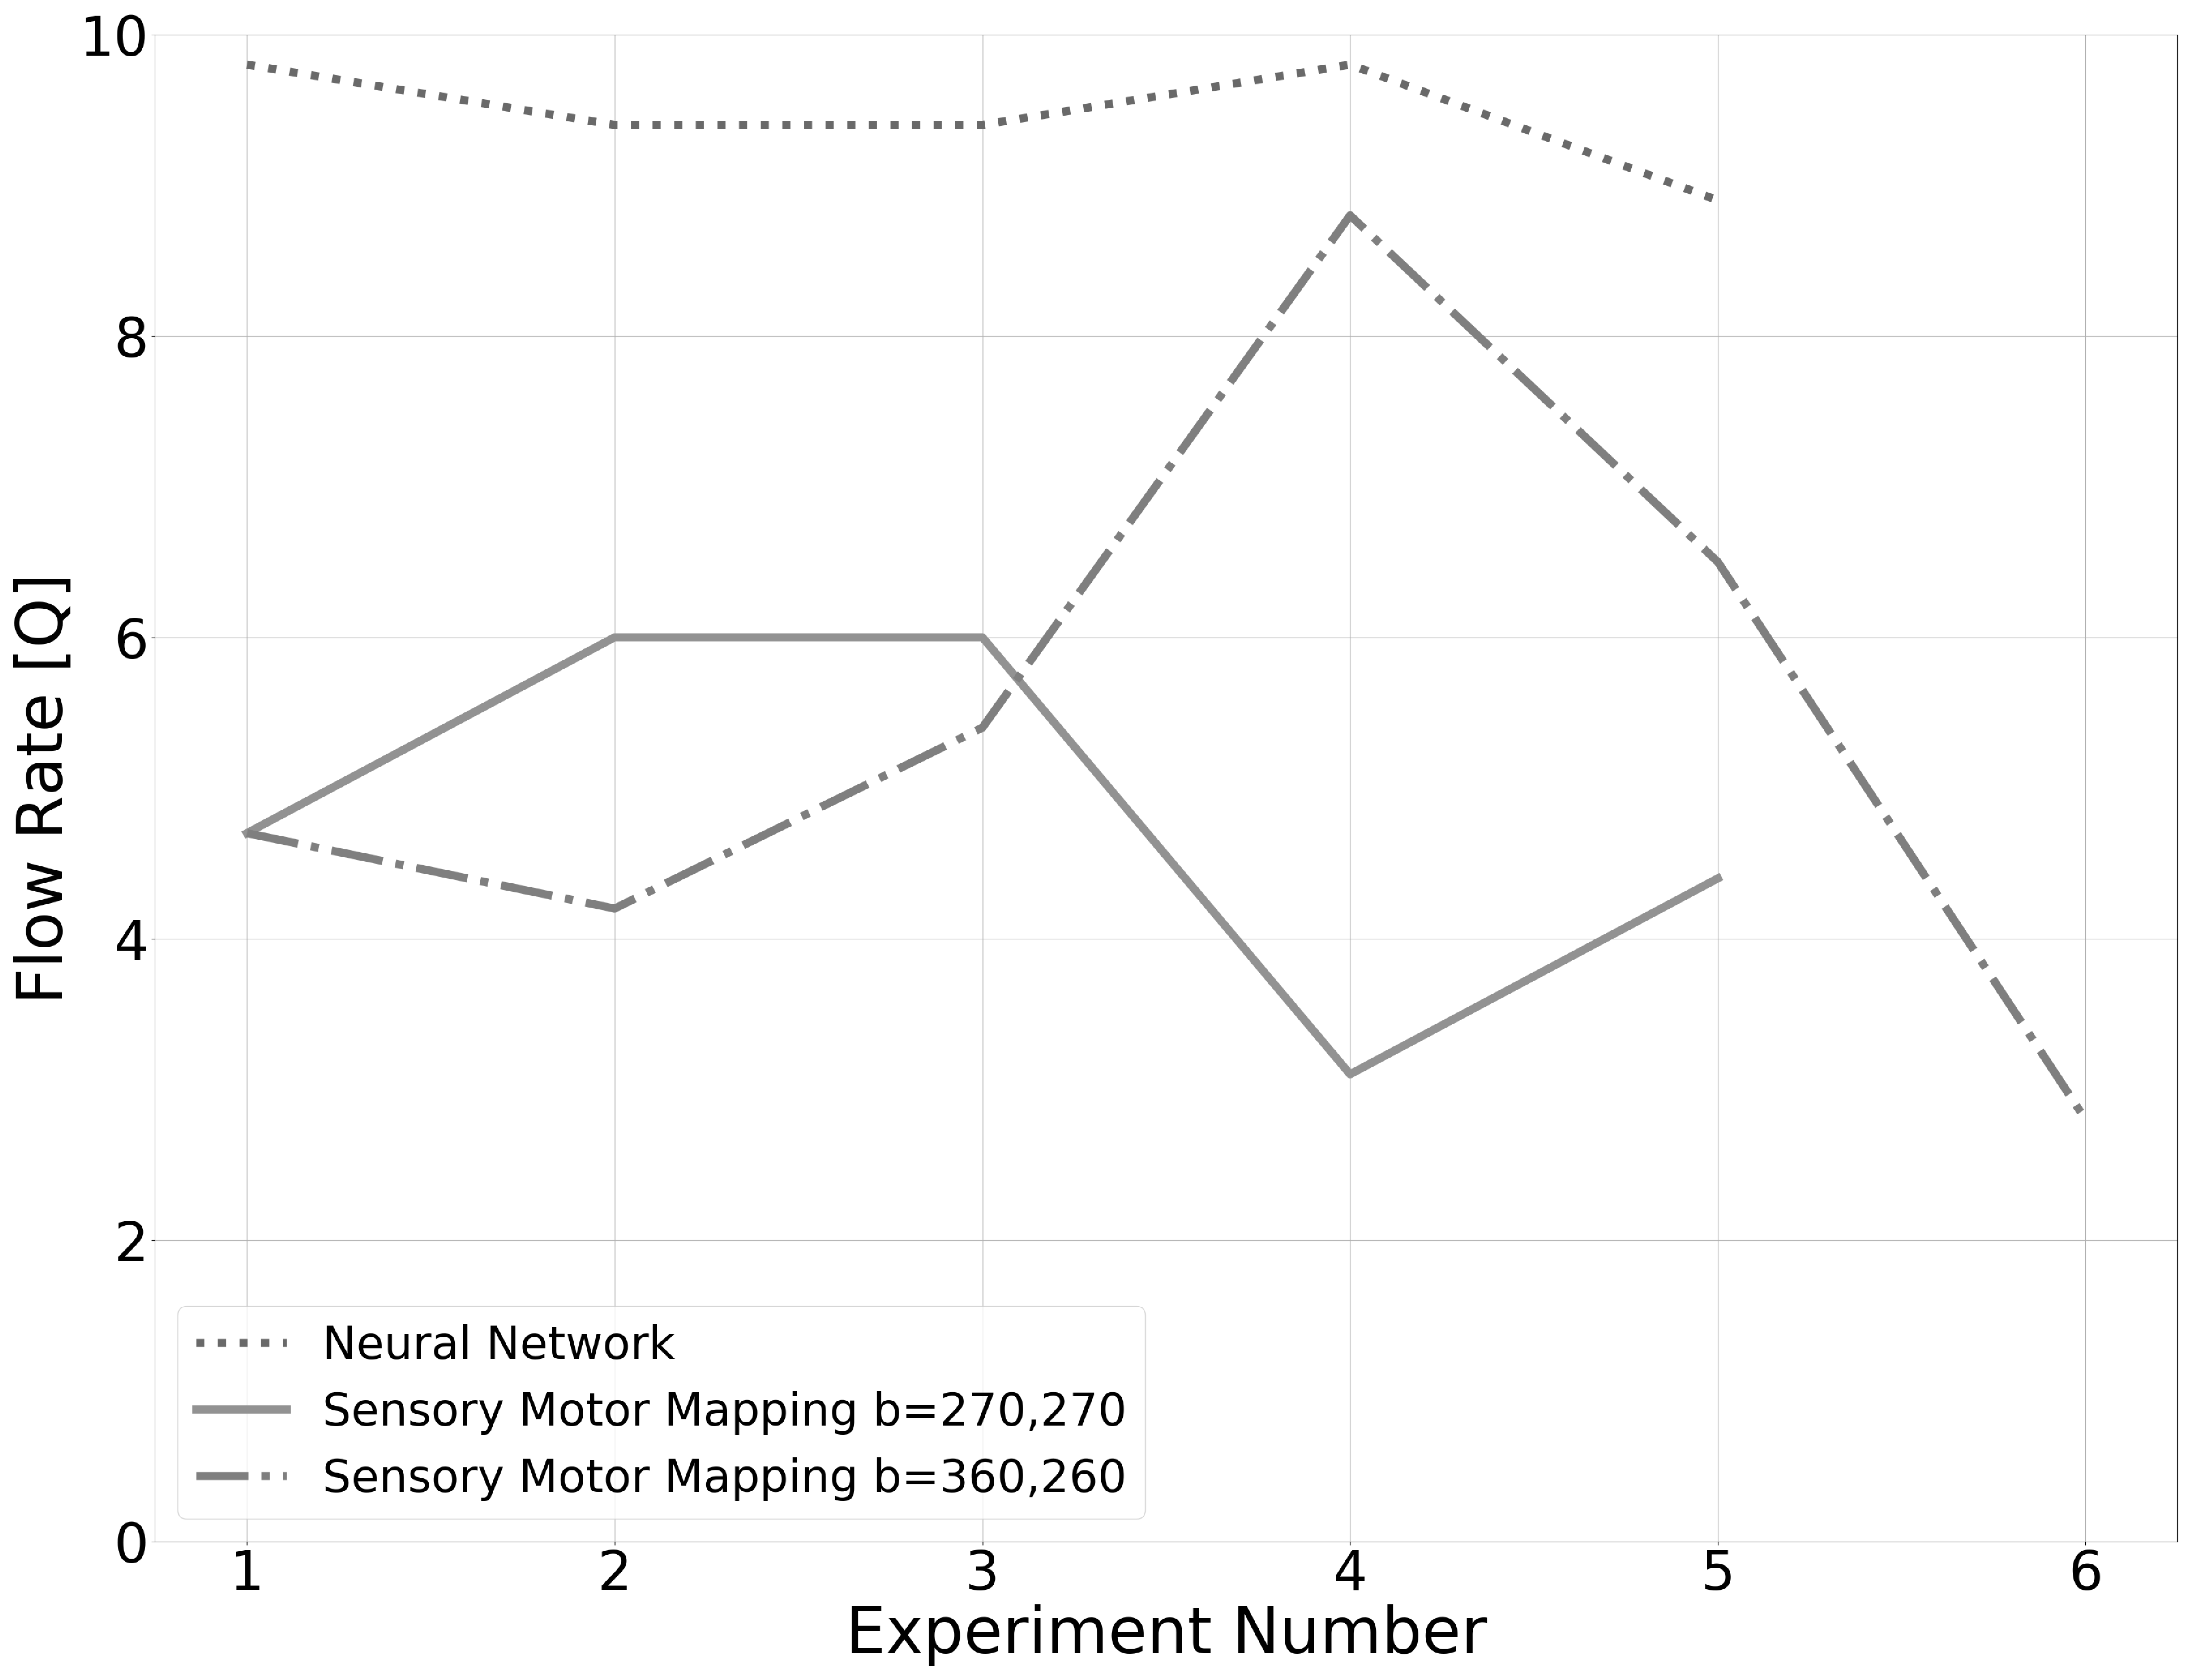
\includegraphics[width=0.9\linewidth]{result_diagrim_rand.eps}
    \caption{ランダムの初期配置で実験回数により流量の変化図}
    \label{random_result}
\end{figure}


\vspace{-1mm}
\begin{figure}[!ht]
    \centering
    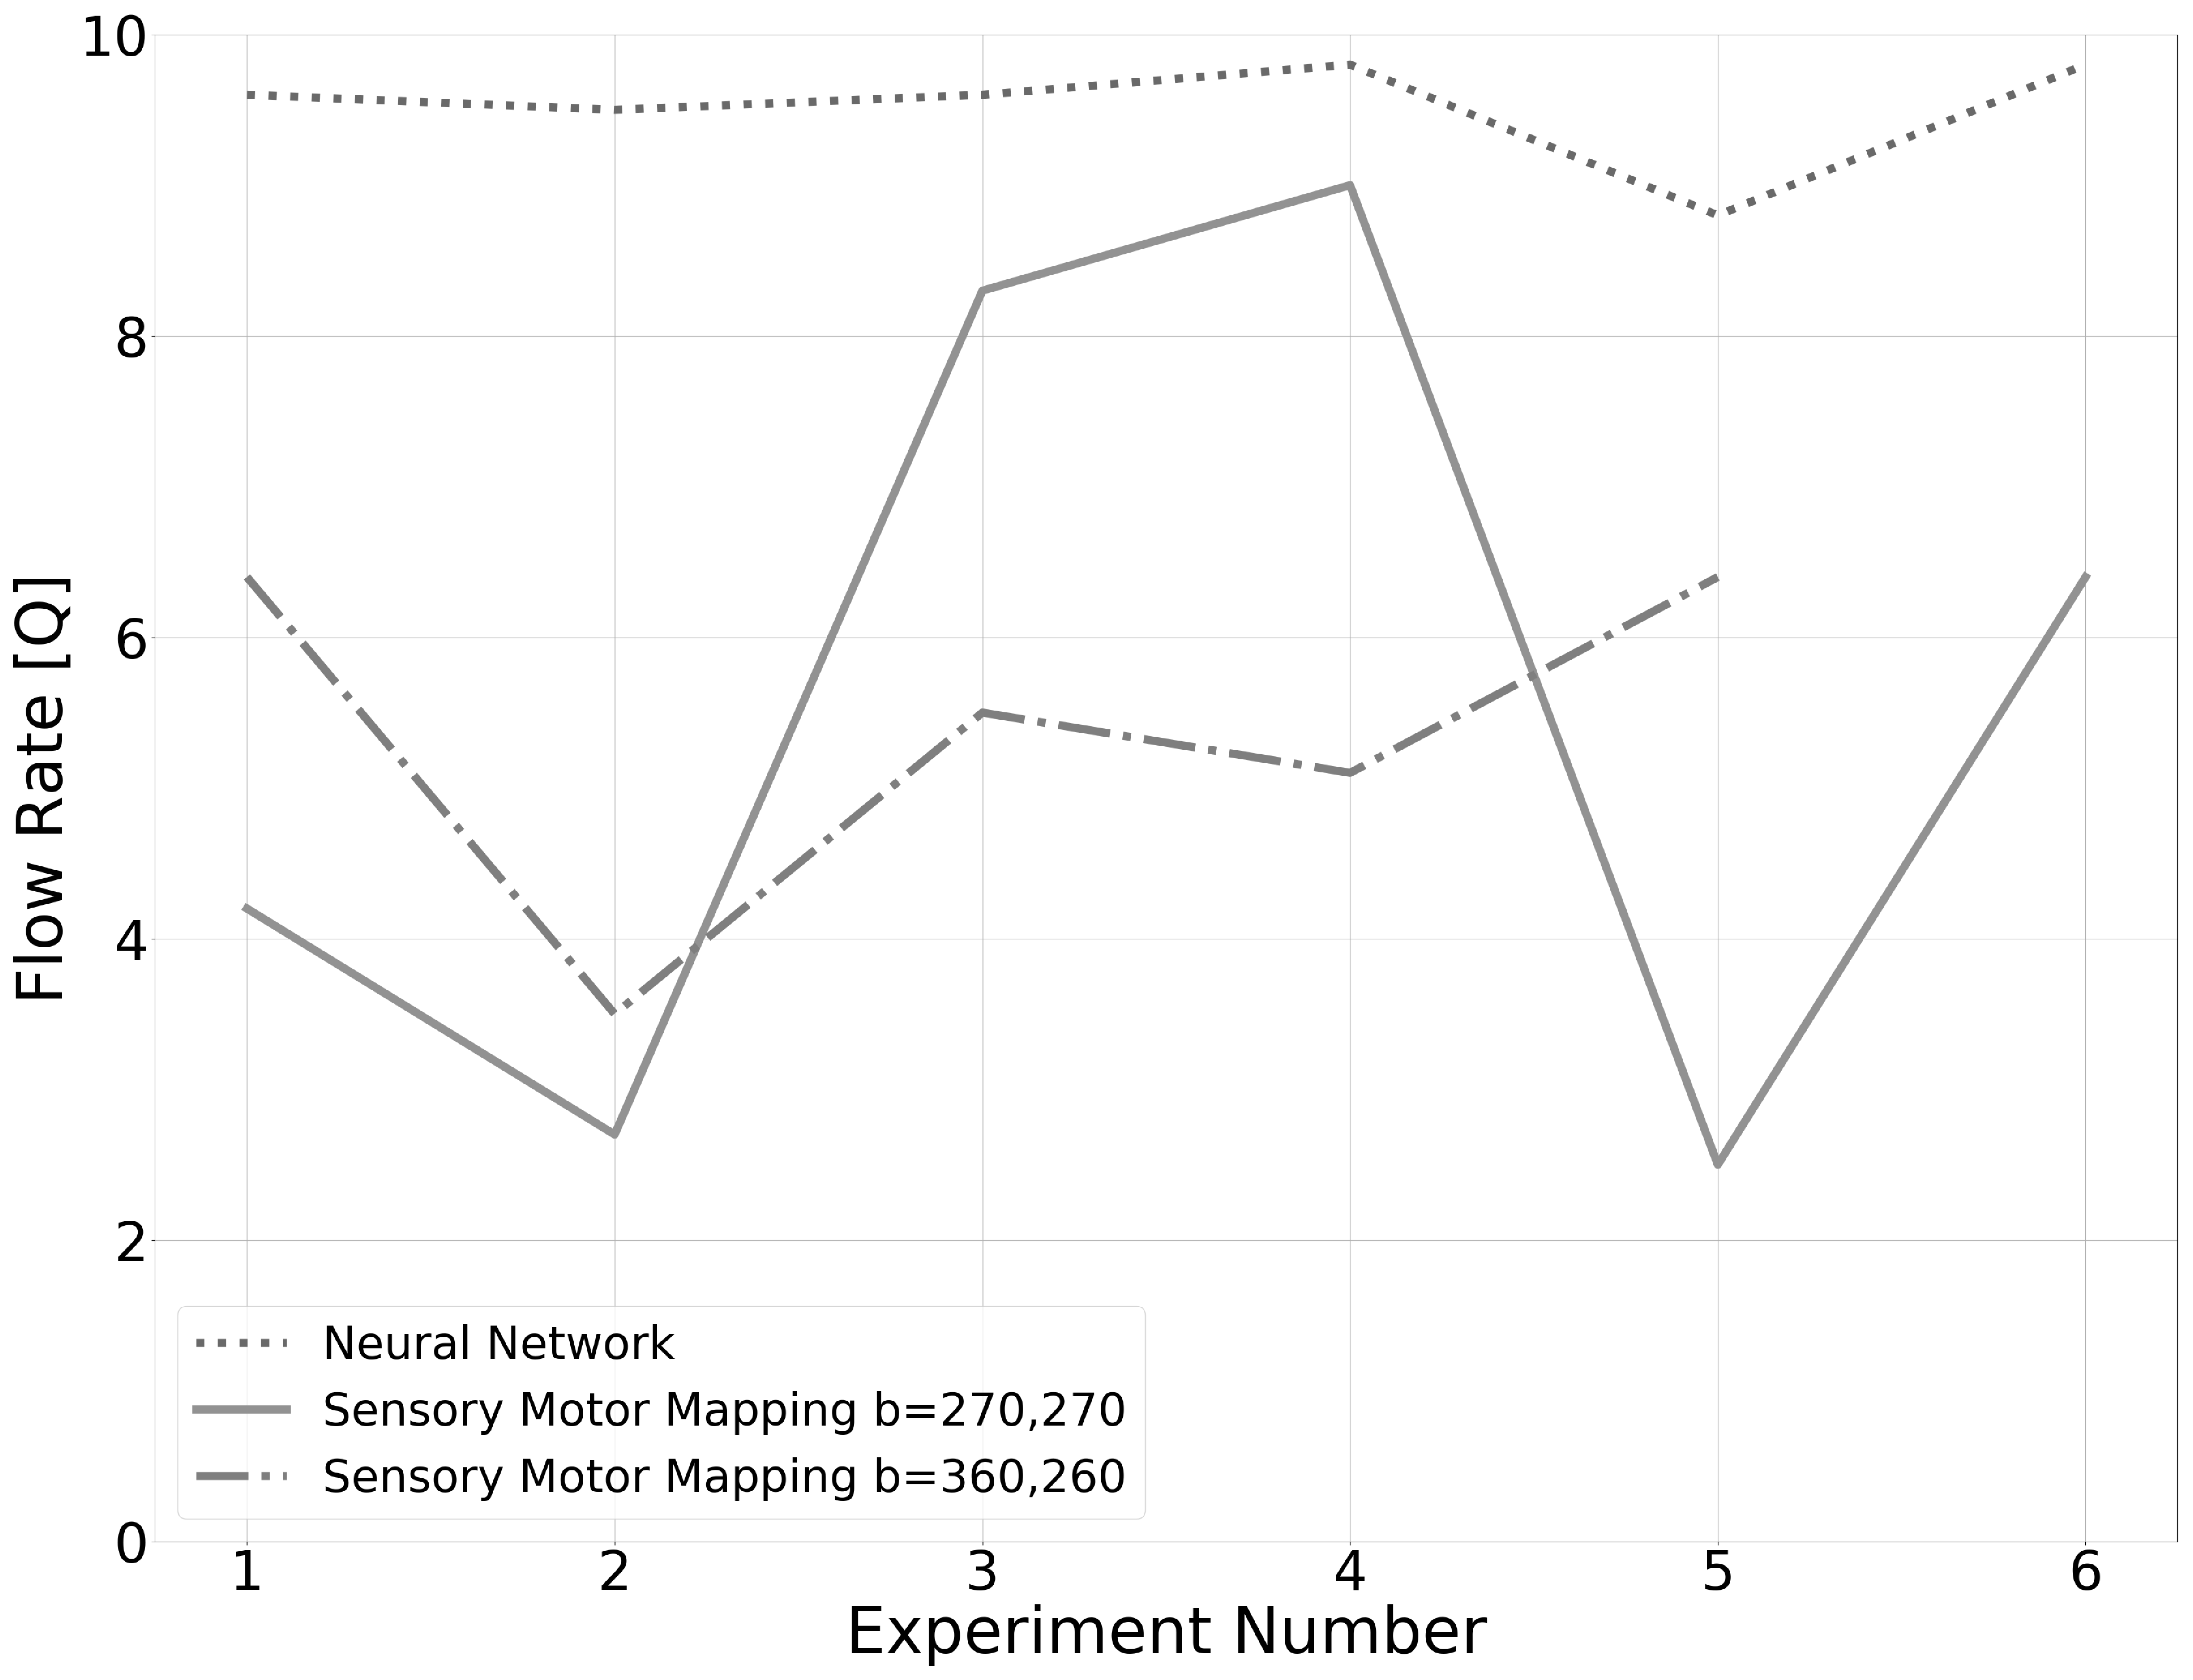
\includegraphics[width=0.9\linewidth]{result_diagrim_crow.eps}
    \caption{渋滞の初期配置で実験回数により流量の変化図}
    \label{crowd_result}
\end{figure}


\vspace{-1mm}
\begin{figure}[!ht]
    \centering
    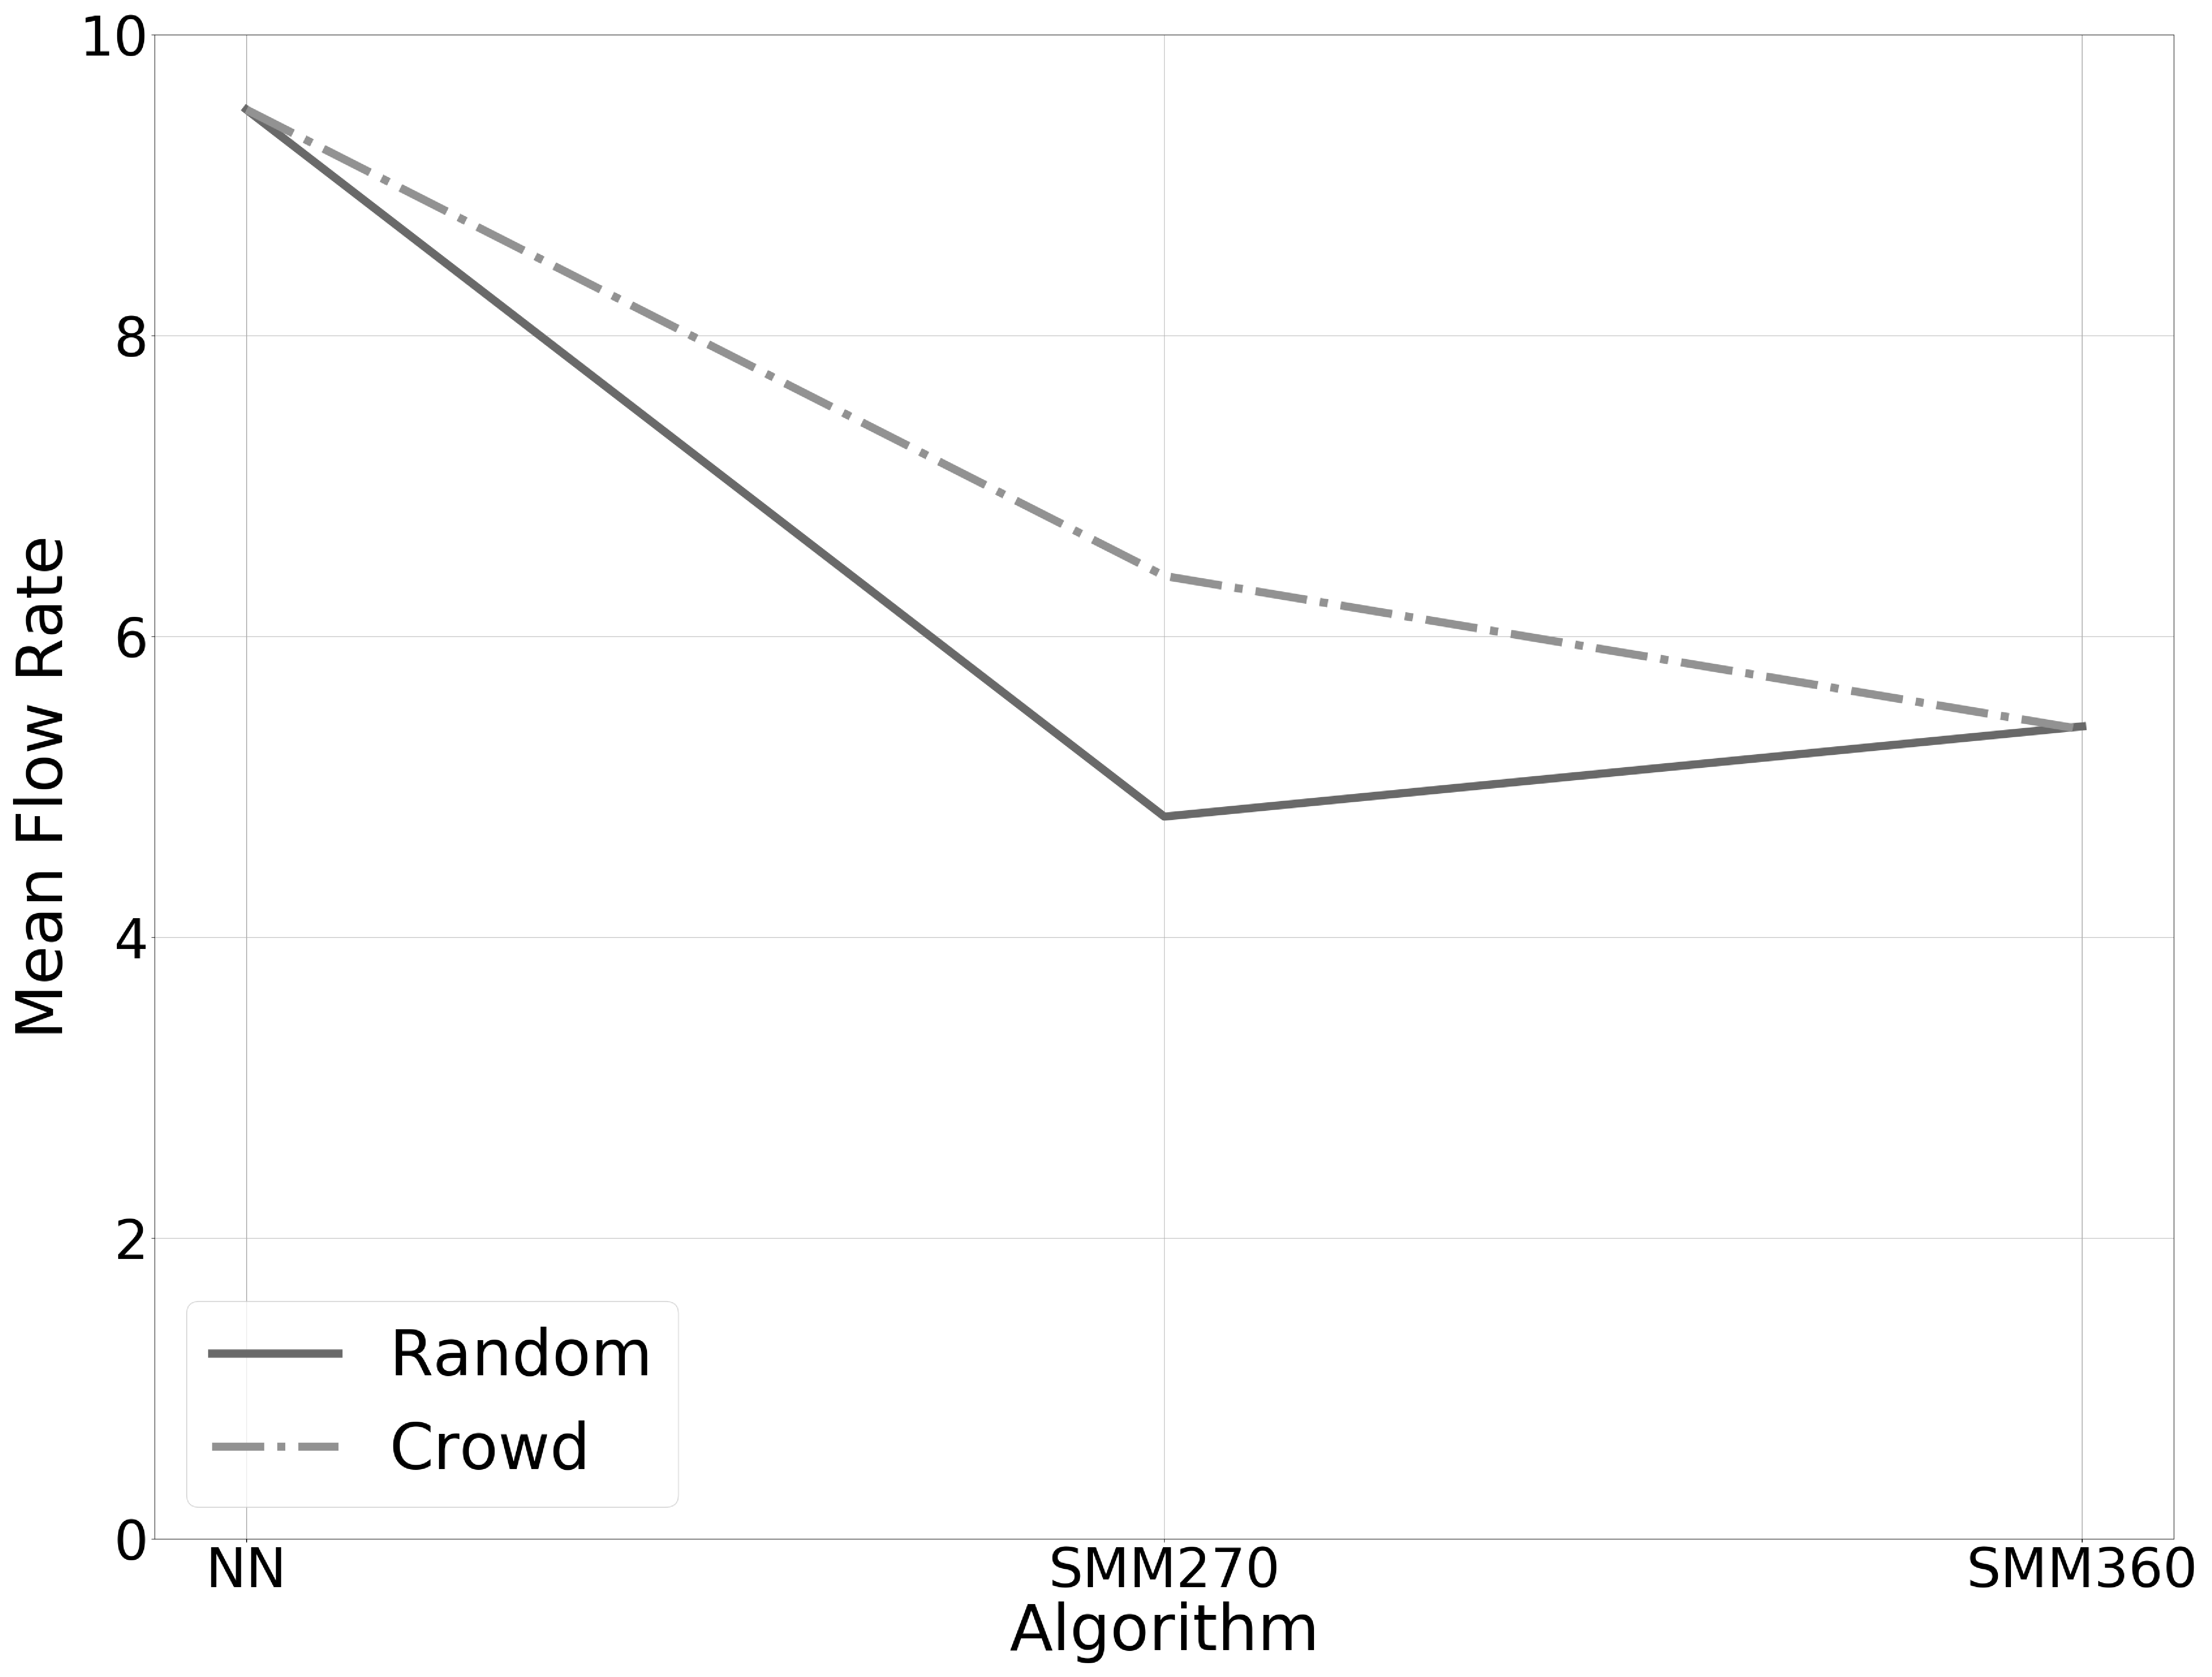
\includegraphics[width=0.9\linewidth]{mean_Q.eps}
    \caption{異なるアルゴリズムの平均流量の比較}
    \label{compare_result}
\end{figure}

\section{まとめ}
1次元画像データ認識ニューラルネットワークより8台ロボットが縞模様のコースで対面走行ができると確認した.
感覚運動写像と比べて,方向転換教えなくても,対面走行を維持する能力が高い.

本文説明した対面走行維持できるニューラルネットワークの学習結果は,著者が何十回練習して,経験を踏まえ,ラジコンする時,遠くから曲がる,近づいて曲がる,真正面にロボットや壁ある時後退することをわざわざ人間の意識持ってロボットに教えて収集した教師データの学習結果です,研究室の他の人がラジコンして収集した教師データも学習して,自律走行の質もそれぞれだ.それに,コースの壁の代わりに,別のもの(ダンボール,雑誌,サンダルなど)を配置して,収集した教師データの学習結果では自律走行ができないことが観察された,その原因として,画像を列ずつ足し算してもらった1次元画像データが障害物と通路の特徴を失って,区別できなくなると考える.

今後の展望として,色んな教師データの違いと特徴をを分析して,どんな教師データがあれば対面走行維持できるを解明すると教師データの質を評価方法を開発する必要がある.
また,画像エントロピーで環境の複雑度を評価して1次元画像データの限界を解明すると考える.


\begin{thebibliography}{9}
\bibitem{asada} 浅田稔,国吉康夫「ロボットインテリジンス」(2006).
\bibitem{li} 李 方 正, 橋爪晋平, 本田泰.「非線形感覚運動写像ロボットの対面流–1 方向走行流への転移と流量のコース幅依存性–」第26回交通流と自己駆動粒子系シンポジウム論文集 (2020)
\end{thebibliography}
\end{document}
